\documentclass{beamer}

\usetheme{Madrid}
\usepackage[utf8]{inputenc}
\usepackage{default}
\usepackage{graphicx}
\usepackage{setspace}
\usepackage{algorithm,algorithmic}
\usepackage{amssymb}
\usepackage{tabularx}
\usepackage{caption}
\usepackage{wasysym}
\usepackage{soul}
\usepackage{textcomp}


\newcommand\good{{\color{green}\DejaSans ☺}}
\newcommand\neutral{{\color{blue}\DejaSans 😐}}
\newcommand\bad{{\color{red}\DejaSans ☹}}
\makeatletter
\newcommand\SoulColor{%
  \let\set@color\beamerorig@set@color
  \let\reset@color\beamerorig@reset@color}
\makeatother

\newcommand*\MyPitem{%
  \item[\color{green}\scalebox{0.9}{\textbullet}]}
\newcommand*\MyCitem{%
  \item[\color{red}\scalebox{0.9}{\textbullet}]}

\AtBeginSection[]
{
\begin{frame}<beamer>
\frametitle{Outline}
\tableofcontents[currentsection]
\end{frame}
}

\title{Numerical Relation Extraction from the Web}
\subtitle{MTP Stage 1 Presentation}
\author[]{Aman Madaan \and Ashish Mittal}
\institute[]{
  Indian Institute of Technology Bombay, Mumbai
}
\date{22nd October, 2014}
\begin{document}
\maketitle
\section{Motivation}

%PART 1 : Motivation
\begin{frame}{Entities have Numerical Attributes}

    \begin{figure}
    \centering
    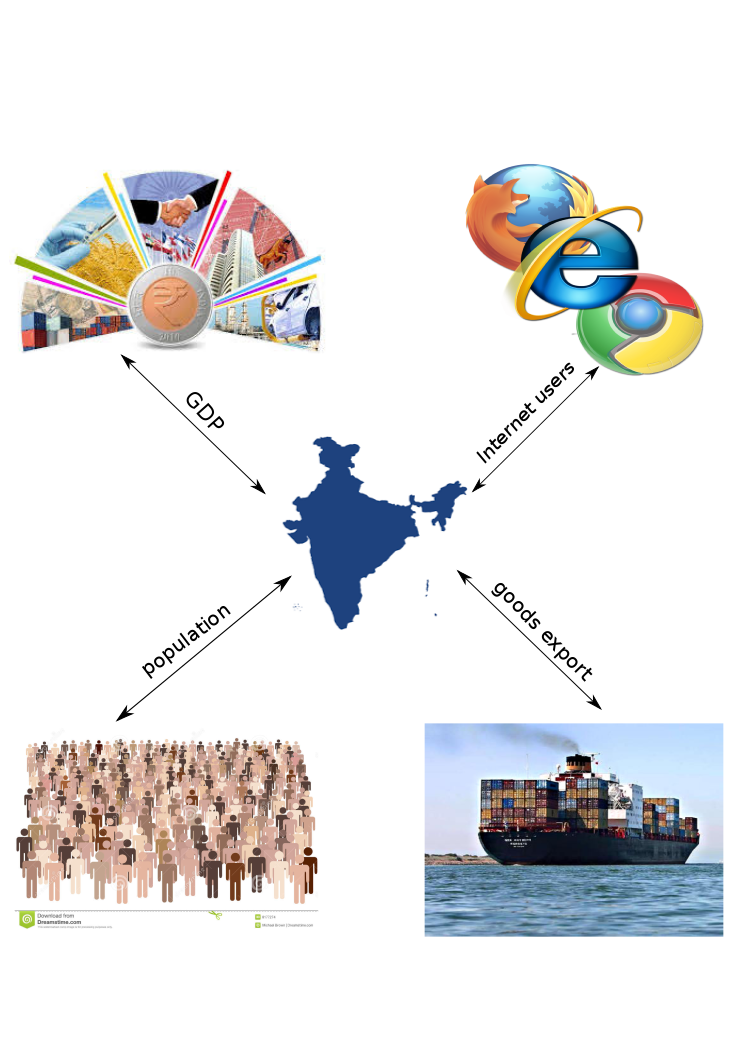
\includegraphics[width = 0.5\textwidth]{images/motivation}
  \end{figure}
 
\end{frame}

\begin{frame}{Entities have Numerical Attributes}
 \begin{center}
 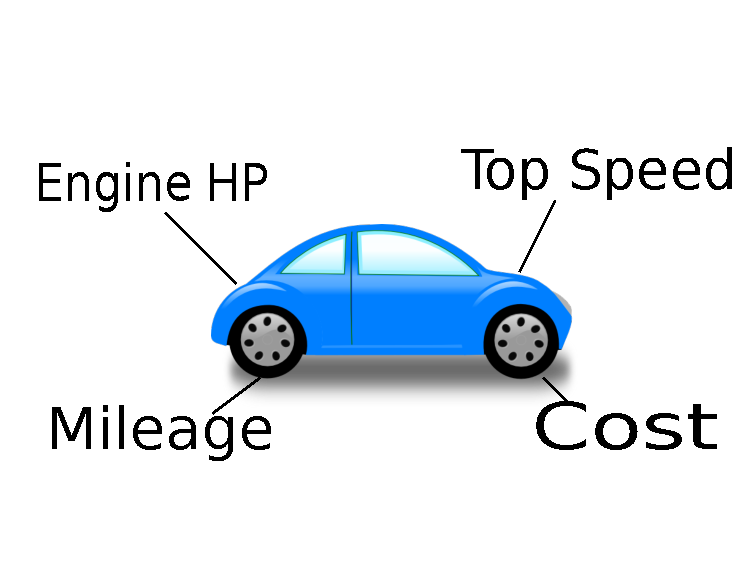
\includegraphics[scale=0.45]{./imgs/car.pdf}
 % car.pdf: 363x272 pixel, 72dpi, 12.81x9.60 cm, bb=0 0 363 272
\end{center}

\end{frame}

\begin{frame}{Entities and Numerical Attributes}
 
 \begin{itemize}

  \item For popular entities, finding complete knowledge bases is possible. \pause \\~\\
  \item data.worldbank.org, Wikipedia infoboxes, freebase ... \pause \\~\\
  \item What about less popular entities?  \pause 
    \begin{itemize}
      \item What is the population of Arbit Apartments, Powai? \pause \\~\\
      \item What is the GDP of Sugarcane Industry of India? \pause \\~\\
      \item Percent of Internet users in Mumbai? 
    \end{itemize}
 \end{itemize} 
\end{frame}

\begin{frame}{Motivation}
 \begin{figure}[h]
 \centering
 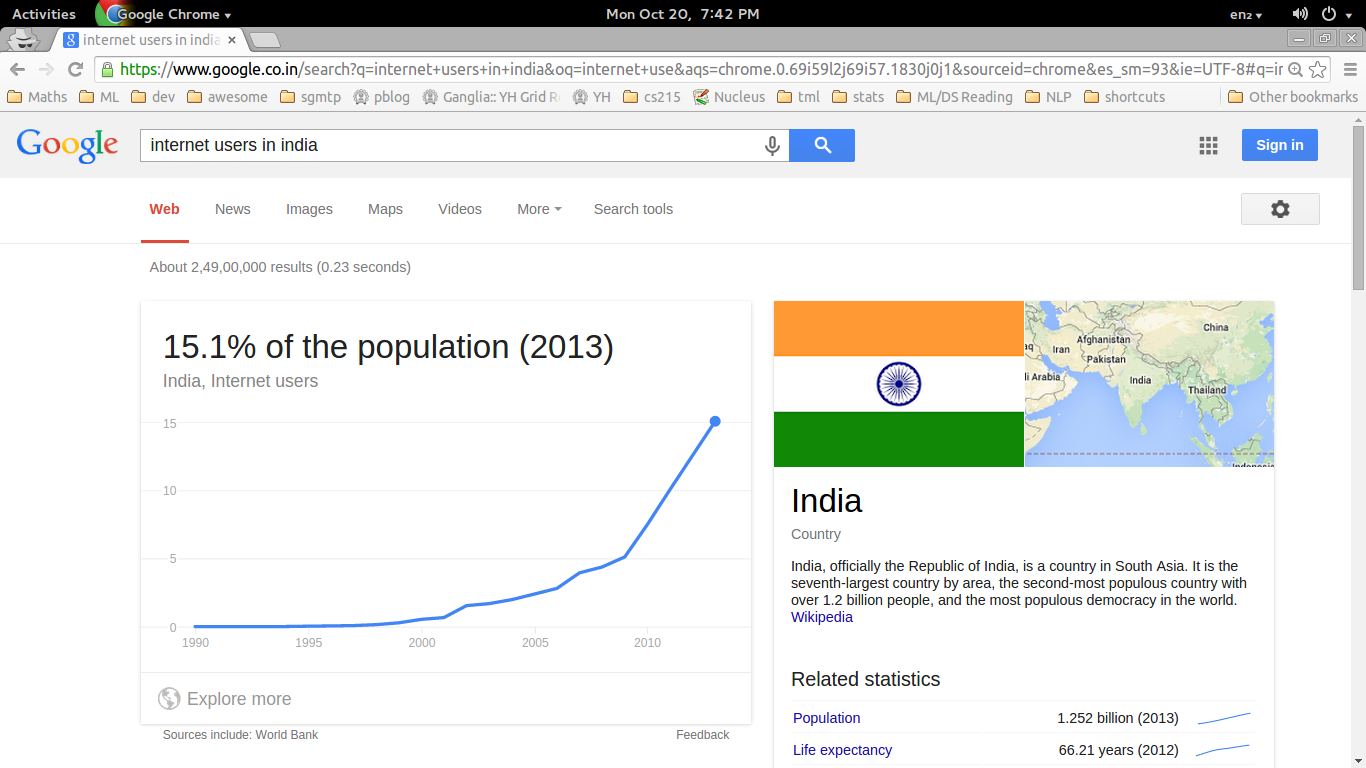
\includegraphics[bb=0 0 1366 741,scale=0.25]{./imgs/resultindia.png}
 % resultindia.png: 1366x741 pixel, 72dpi, 48.19x26.14 cm, bb=0 0 1366 741
\end{figure}
\end{frame}

\begin{frame}{Motivation}
 \begin{figure}[h]
 \centering
 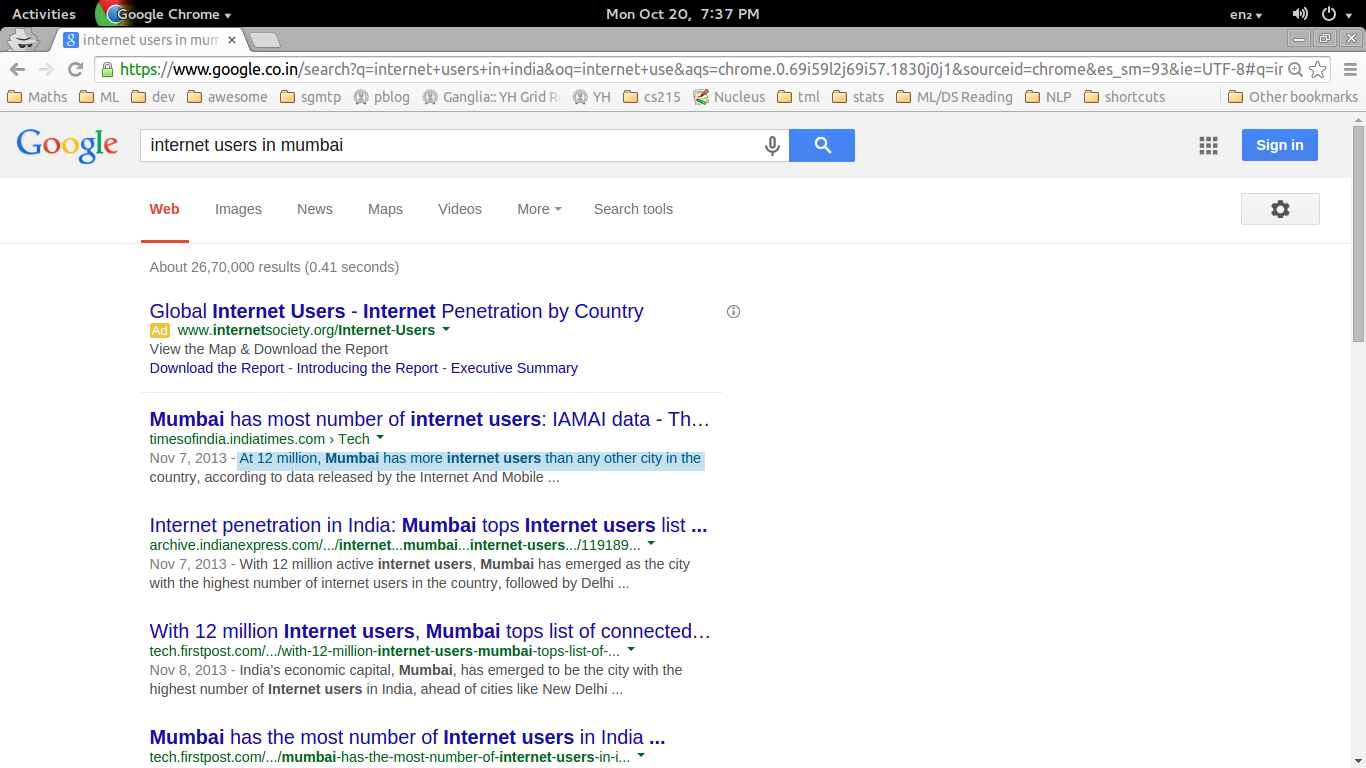
\includegraphics[bb=0 0 1366 741,scale=0.25]{./imgs/resultmumbai.png}
 % resultindia.png: 1366x741 pixel, 72dpi, 48.19x26.14 cm, bb=0 0 1366 741
\end{figure}
\end{frame}

\begin{frame}{Motivation}

\begin{itemize}
 \item  Web is huge.  \pause \\~\\
 \item Probably, there is some page which contains the information we are looking for. \pause \\~\\
 \item The way in which you express a fact about an entity depends on the fact, and not the entity. \pause \\~\\
 \item We may expect \textbf{the sentence structure} \footnote{More on this in the coming slides} to be similar. \pause
 \begin{itemize}
    \item Population of India reached 1.3 billion, making it the second largest country in the world. \pause \\~\\
    \item Population of Arbit Apartments, Powai reached 1300.
 \end{itemize}
 
\end{itemize}
\end{frame}



\section{Problem Statement}
\begin{frame}{Problem Statement}
 \begin{itemize}
  \item Given that we know a lot of facts about some entities, can we train extractors that run over the web and pull similar facts about other entities?
 \end{itemize}
\end{frame}
\begin{frame}{Problem Statement}

\begin{itemize}
 
 \item  The knowledge is scattered in unstructured text on the Web.
 \begin{figure}[h]
 \centering
 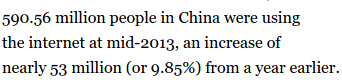
\includegraphics[bb=0 0 1139 53,scale=0.47]{./images/ex_2.png}
 % ex_1.png: 1139x53 pixel, 72dpi, 40.18x1.87 cm, bb=0 0 1139 53
\end{figure}

 \begin{figure}[h]
 \centering
 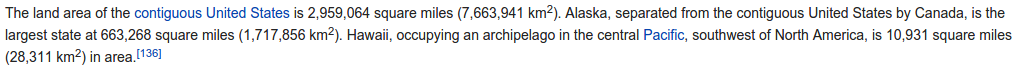
\includegraphics[bb=0 0 1139 53,scale=0.30]{./images/ex_3.png}
 % ex_1.png: 1139x53 pixel, 72dpi, 40.18x1.87 cm, bb=0 0 1139 53
\end{figure}


  \item Can such facts be extracted automatically?
\end{itemize}

\end{frame}
\begin{frame}{Problem Statement}
\begin{itemize}
 \item Formally, train extractors that can harness the Web for numerical relations, where relations are 3-tuples linking an entity
to a number \\~\\
   
    \begin{itemize}
	\item  (India, \textbf{economy}, 1.842 trillion USD) \\~\\
	\item  (China, \textbf{internet users},  590.56 million) \\~\\
	\item  (USA, \textbf{land area}, 2,959,054 square mile)
    \end{itemize}

 \end{itemize}
\end{frame}

%PART 2 : Relation extraction as a machine learning problem

\section{Relation Extraction as a Machine Learning Problem}

\begin{frame}{Relation Extraction as a Machine Learning Problem}
 \begin{itemize}
  \item \textbf{Structure} and \textbf{content} of sentences expressing the same relations can be \emph{expected} to be similar.  \\~\\
 \begin{itemize}
      \item The population of Australia is estimated to be 23,622,400 as of 7 October 2014. \\~\\
      \item According to an official estimate for 1 June 2014, the population of Russia is 143,800,000.   
   \end{itemize}   
 \end{itemize}
\end{frame}
\begin{frame}{Relation Extraction as a Machine Learning Problem}
\begin{itemize}
\item \textbf{Structure} and \textbf{content} of sentences expressing the same relations can be \emph{expected} to be similar.  \\~\\
 \begin{itemize}   
    \item At 17,075,400 square kilometres, Russia is the largest country in the world. \\~\\
    \item With an area of 504,030 $km^{2}$, Spain is the second largest country in Western Europe. 
    \end{itemize}
 \end{itemize}
\end{frame}
\begin{frame}{Relation Extraction as a Machine Learning Problem}
 
 \begin{itemize}
  \item Redundancy in grammatical features and dependencies of the sentences expressing same relation. \pause 
     \begin{figure}
    \centering
    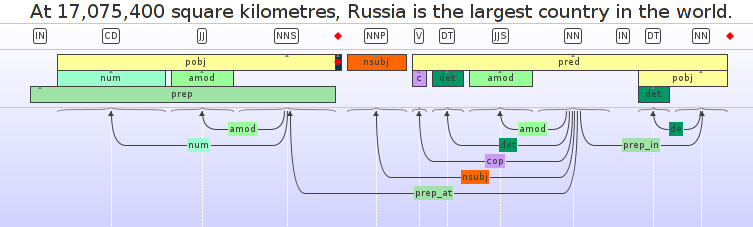
\includegraphics[width = 0.8\textwidth]{images/ex_4}
  \end{figure} \pause
  
   \begin{figure}
    \centering
    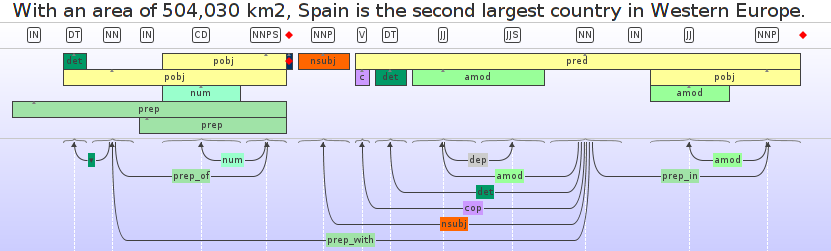
\includegraphics[width = 0.8\textwidth]{images/ex_5}
  \end{figure}
 \end{itemize}

\end{frame}



\begin{frame}{Possible Workflow} \pause
\begin{algorithm}[H]
\setstretch{1.35}
\begin{algorithmic}[1]
\STATE \textbf{Collect enough examples} for each relation so that there are sufficient patterns and enough redundancy to exploit. \\ \pause
\STATE \textbf{Extract features} (important keywords, grammatical structure, parse trees, etc.) for these sentences. \\ \pause
\STATE \textbf{Train} a multi-class classifier on this training data. \\ \pause
\FOR{$sentence\ s \in Corpus $} \pause
\STATE \textbf{Extract} features for $s$. \pause
\STATE \textbf{Predict} the relation using the model for these features. \pause
\STATE \textbf{Store} the fact into a database.
\ENDFOR

\end{algorithmic}
\caption*{Relation Extraction}
\label{alg:seq}
\end{algorithm}
\end{frame}

\begin{frame}{Challenge}
 \begin{itemize}
  \item Large Corpus ($\sim$16 million sentences), hand labeling is out of question \pause \\~\\
  \item Need lots of training data to learn high quality extractors \pause \\~\\
  \item Is there a middle ground?
 \end{itemize}
\end{frame}

\section{Distant Supervision}
%PART 3 DS
\begin{frame}{Distant Supervision} \pause 
\begin{itemize}
 
 \item  \emph{Weak} Supervision\pause \\~\\
  \item Use Heuristics to \textbf{align} a \textbf{table} of facts with the \textbf{corpus}  \pause \\~\\
  \item \emph{Fuzzy} training data 
  
\end{itemize}
\end{frame}

\begin{frame}{Distant Supervision}{Example}
\begin{itemize}
 
\item Born - In database
 \begin{center}
\begin{tabular}{|l|l|}
\hline
Donald Knuth & Wisconsin \\
Srinivasa Ramanujan & Erode \\
Alan Turing & London \\
\hline
\end{tabular}
\end{center}
\item Given Sentences
\begin{itemize}
\item Srinivasa Ramanujan was born in his maternal grandmother’s home in Erode.
\item Srinivasa Ramanujan was born in Erode, Tamilnadu, India, on 22nd December, 1887.
\item Turing's father was with the Indian Civil Service (ICS) at Chhatrapur, Bihar.
\item Alan Turing biopic The Imitation Game named as London film festival opener.
\end{itemize}
\end{itemize}
 
\end{frame}
\begin{frame}{Distant Supervision}{Example}
\begin{itemize}
 
\item Born - In database
 \begin{center}
\begin{tabular}{|l|l|}
\hline
Donald Knuth & Wisconsin \\
\SoulColor\hl{Srinivasa Ramanujan} & \SoulColor\hl{Erode} \\
Alan Turing & London \\
\hline
\end{tabular}
\end{center}
\item Given Sentences
\setbeamercolor{normal text}{fg=gray,bg=}
\setbeamercolor{alerted text}{fg=black,bg=}
\usebeamercolor{normal text}
\begin{itemize}
\item \alert<+> {\SoulColor\hl{Srinivasa Ramanujan} was born in his maternal grandmother’s home in \SoulColor\hl{Erode}.} \alert{LABEL : BornIn} \checkmark
\item Srinivasa Ramanujan was born in Erode, Tamilnadu, India, on 22nd December, 1887.
\item Turing's father was with the Indian Civil Service (ICS) at Chhatrapur, Bihar.
\item Alan Turing biopic The Imitation Game named as London film festival opener.
\end{itemize}
\end{itemize}
 
\end{frame}
\begin{frame}{Distant Supervision}{Example}
\begin{itemize}
 
\item Born - In database
 \begin{center}
\begin{tabular}{|l|l|}
\hline
Donald Knuth & Wisconsin \\
\SoulColor\hl{Srinivasa Ramanujan} & \SoulColor\hl{Erode} \\
Alan Turing & London \\
\hline
\end{tabular}
\end{center}
\item Given Sentences
\setbeamercolor{normal text}{fg=gray,bg=}
\setbeamercolor{alerted text}{fg=black,bg=}
\usebeamercolor{normal text}
\begin{itemize}
\item Srinivasa Ramanujan was born in his maternal grandmother’s home in Erode.  \checkmark
\item \alert<+> {\SoulColor\hl{Srinivasa Ramanujan} was born in \SoulColor\hl{Erode}, Tamilnadu, India, on 22nd December, 1887.}  \checkmark
\item Turing's father was with the Indian Civil Service (ICS) at Chhatrapur, Bihar.
\item Alan Turing biopic The Imitation Game named as London film festival opener.
\end{itemize}
\end{itemize}
\end{frame}
\begin{frame}{Distant Supervision}{Example}
\begin{itemize}
 
\item Born - In database
 \begin{center}
\begin{tabular}{|l|l|}
\hline
Donald Knuth & Wisconsin \\
Srinivasa Ramanujan & Erode \\
\SoulColor\hl{Alan Turing} & \SoulColor\hl{London} \\
\hline
\end{tabular}
\end{center}
\item Given Sentences
\setbeamercolor{normal text}{fg=gray,bg=}
\setbeamercolor{alerted text}{fg=black,bg=}
\usebeamercolor{normal text}
\begin{itemize}
\item Srinivasa Ramanujan was born in his maternal grandmother’s home in Erode.  \checkmark
\item Srinivasa Ramanujan was born in Erode, Tamilnadu, India, on 22nd December, 1887.  \checkmark
\item \alert<+> {\SoulColor\hl{Turing's} father was with the Indian Civil Service (ICS) at Chhatrapur, Bihar}  \textbf{X}
\item Alan Turing biopic The Imitation Game named as London film festival opener.
\end{itemize}
\end{itemize}
\end{frame}

\begin{frame}{Distant Supervision}{Example}
\begin{itemize}
 
\item Born - In database
 \begin{center}
\begin{tabular}{|l|l|}
\hline
Donald Knuth & Wisconsin \\
Srinivasa Ramanujan & Erode \\
\SoulColor\hl{Alan Turing} & \SoulColor\hl{London} \\
\hline
\end{tabular}
\end{center}
\item Given Sentences
\setbeamercolor{normal text}{fg=gray,bg=}
\setbeamercolor{alerted text}{fg=black,bg=}
\usebeamercolor{normal text}
\begin{itemize}
\item Srinivasa Ramanujan was born in his maternal grandmother’s home in Erode. \checkmark
\item Srinivasa Ramanujan was born in Erode, Tamilnadu, India, on 22nd December, 1887.  \checkmark
\item Turing's father was with the Indian Civil Service (ICS) at Chhatrapur, Bihar.  \textbf{X}
\item \alert<+> {\SoulColor\hl{Alan Turing} biopic The Imitation Game named as \SoulColor\hl{London} film festival opener.} \checkmark
\end{itemize}
\end{itemize}
 
\end{frame}

\begin{frame}{Distant Supervision}{Example}
\begin{itemize}
 
\item Born - In database
 \begin{center}
\begin{tabular}{|l|l|}
\hline
Donald Knuth & Wisconsin \\
Srinivasa Ramanujan & Erode \\
\SoulColor\hl{Alan Turing} & \SoulColor\hl{London} \\
\hline
\end{tabular}
\end{center}
\item Given Sentences
\setbeamercolor{normal text}{fg=gray,bg=}
\setbeamercolor{alerted text}{fg=black,bg=}
\usebeamercolor{normal text}
\begin{itemize}
\item Srinivasa Ramanujan was born in his maternal grandmother’s home in Erode.   \checkmark
\item Srinivasa Ramanujan was born in Erode, Tamilnadu, India, on 22nd December, 1887.   \checkmark
\item Turing's father was with the Indian Civil Service (ICS) at Chhatrapur, Bihar. \textbf{X}
\item \alert<+> {\SoulColor\hl{Alan Turing} biopic The Imitation Game named as \SoulColor\hl{London} film festival opener.\checkmark {\color{red}FALSE POSITIVE}} 
\end{itemize}
\end{itemize}
 
\end{frame}

\begin{frame}{Distant Supervision} \pause
\begin{itemize}
\item[\textcolor{red}{$\bullet$}] \emph{Distant supervision assumption:} If an entity pair $E$ appears with a relation $R$ in the knowledge base, then any sentence containing $E$ \textbf{will} express $R$ \pause \\~\\
\item[\textcolor{green}{$\bullet$}] Can quickly label huge corpora \pause \\~\\
\item[\textcolor{red}{$\bullet$}] Same entity pair can match different relations (Founded(Steve Jobs, Apple) or CEO(Steve Jobs, Apple)) \pause \\~\\
\item[\textcolor{red}{$\bullet$}] False positives, may lead to the model learning wrong patterns for relations (E.g. ``Film Festival'' an Indicator of BornIn) 
\end{itemize}
\end{frame}

\section{Distant Supervision Techniques}
%PART 4: MultiR
\begin{frame}{Distant Supervision Techniques}
 \begin{itemize}
  \item First paper in 1999, almost every possibility explored
 \end{itemize}
\begin{center}
 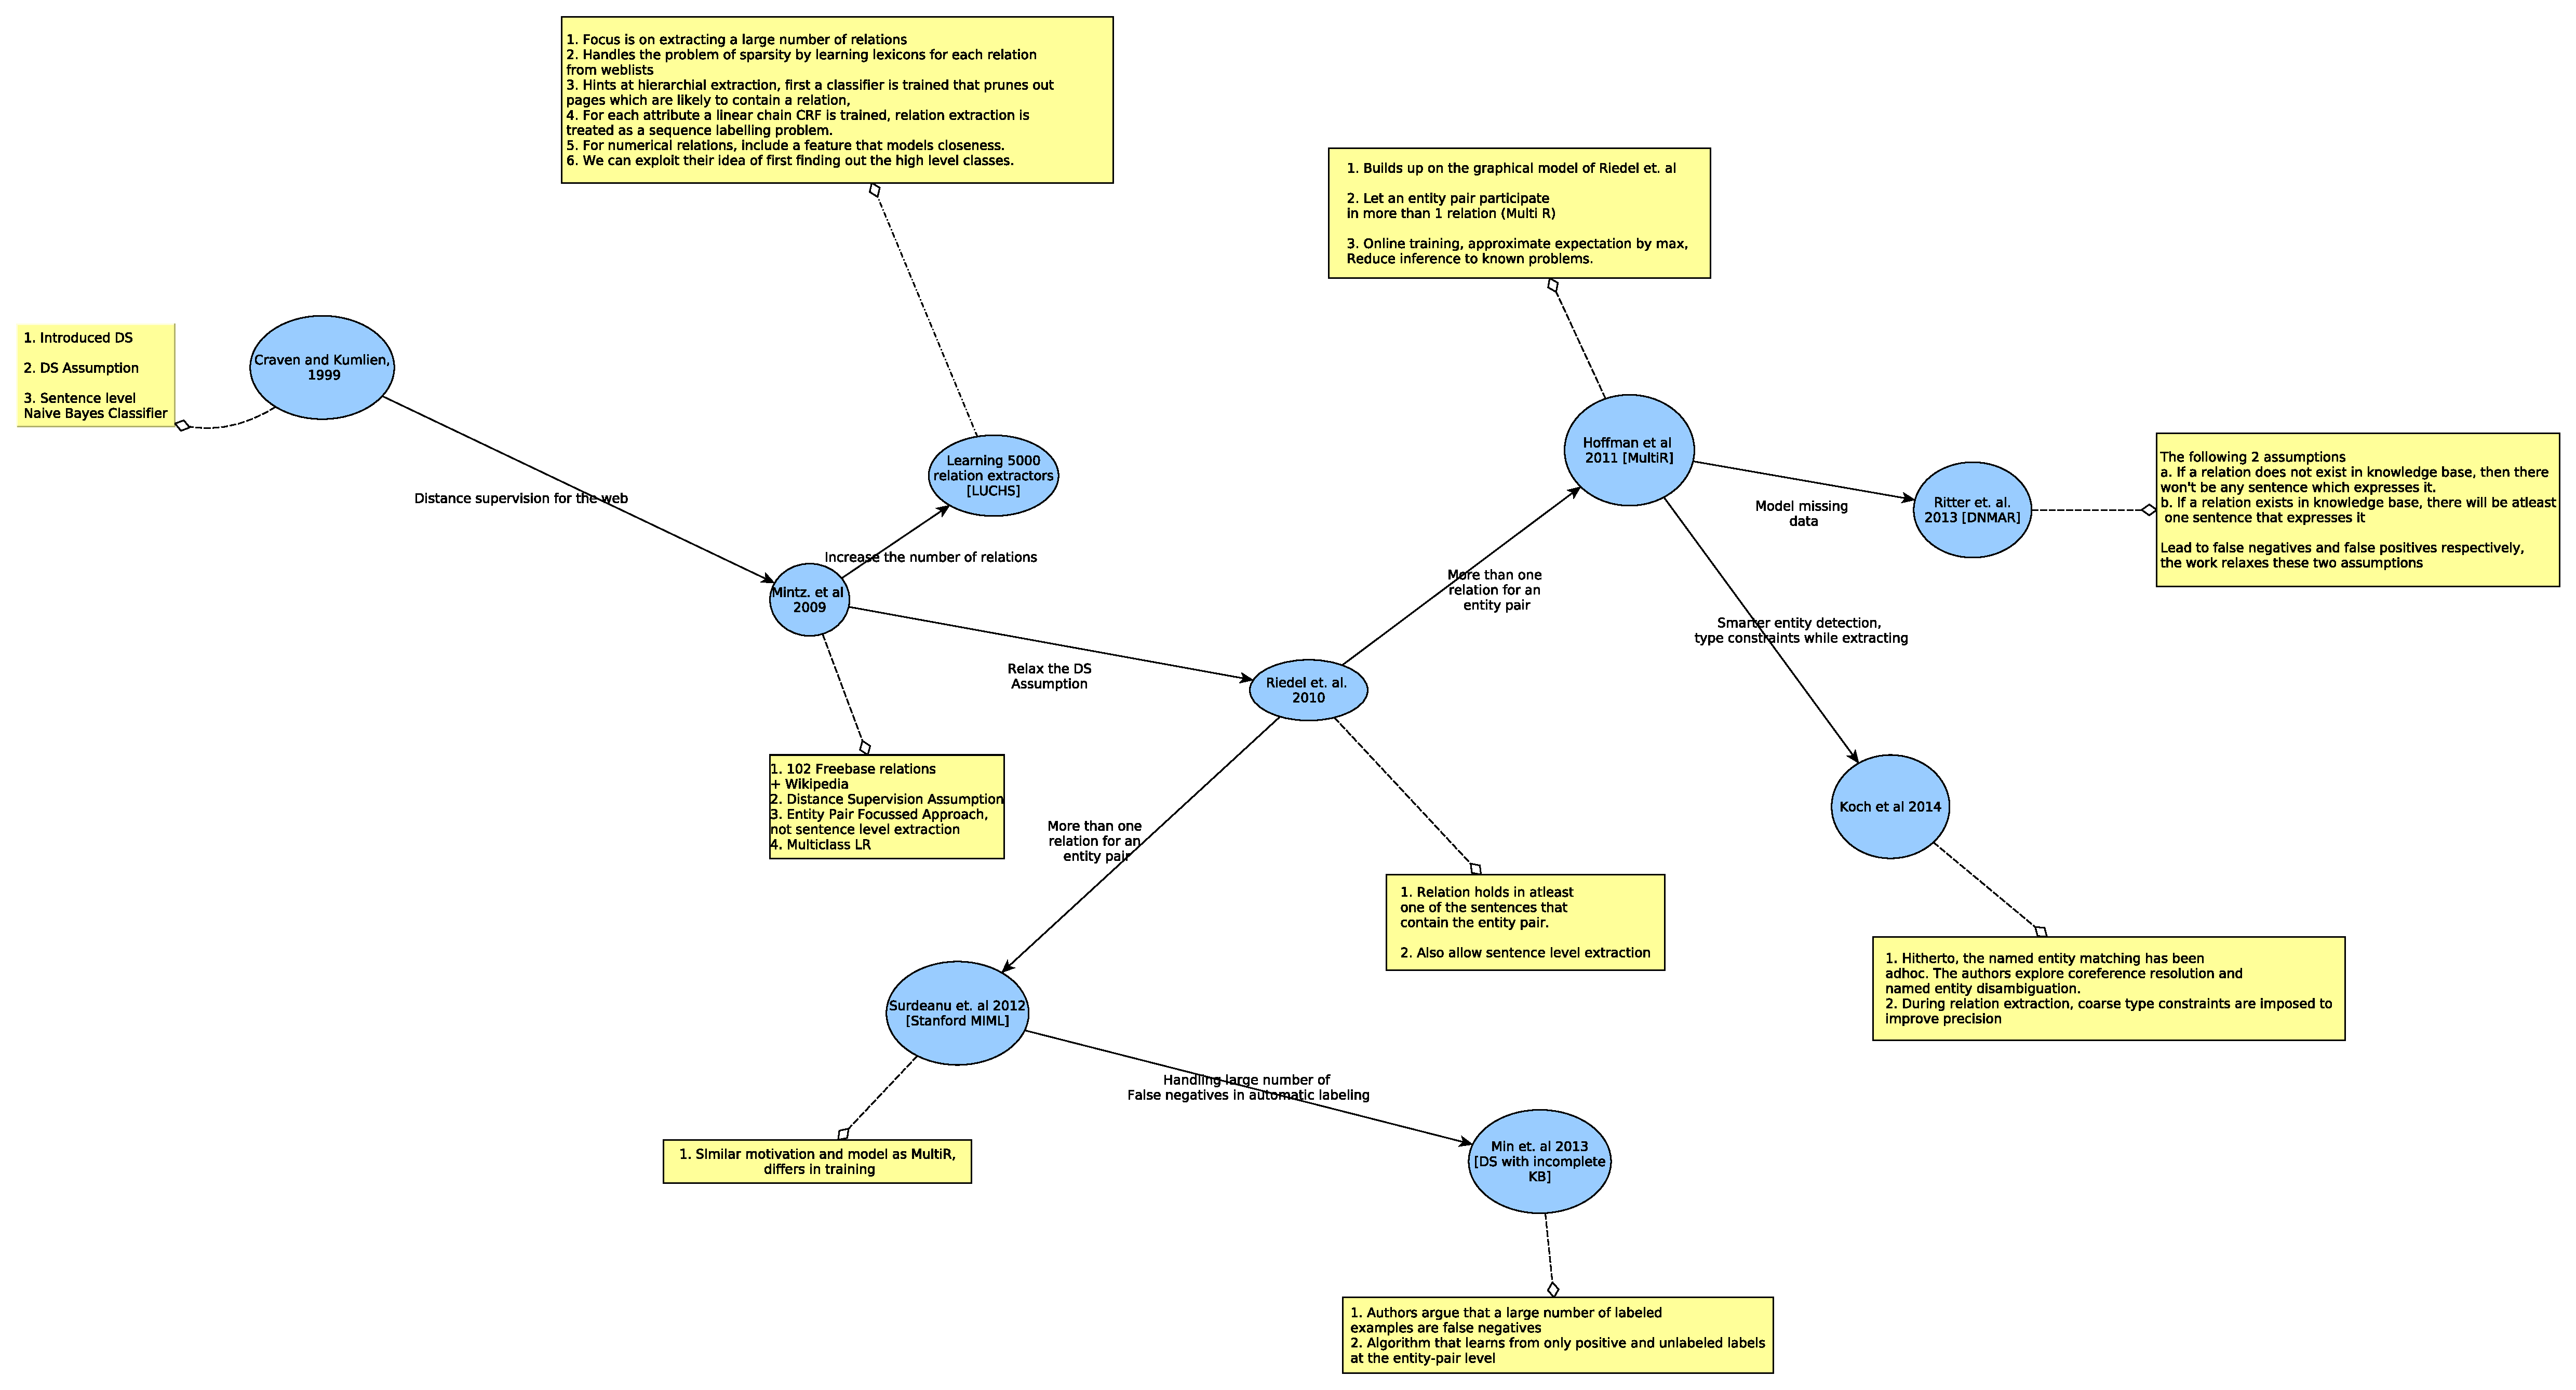
\includegraphics[scale=0.12]{./imgs/dsreadings.pdf}
 % dsreadings.pdf: 2381x1285 pixel, 72dpi, 84.00x45.33 cm, bb=0 0 2381 1285
\end{center}
\end{frame}
\begin{frame}{Distant Supervision Techniques}
 \begin{itemize}
  \item First paper in 1999, \emph{almost} every possibility explored
 \end{itemize}
\begin{center}
 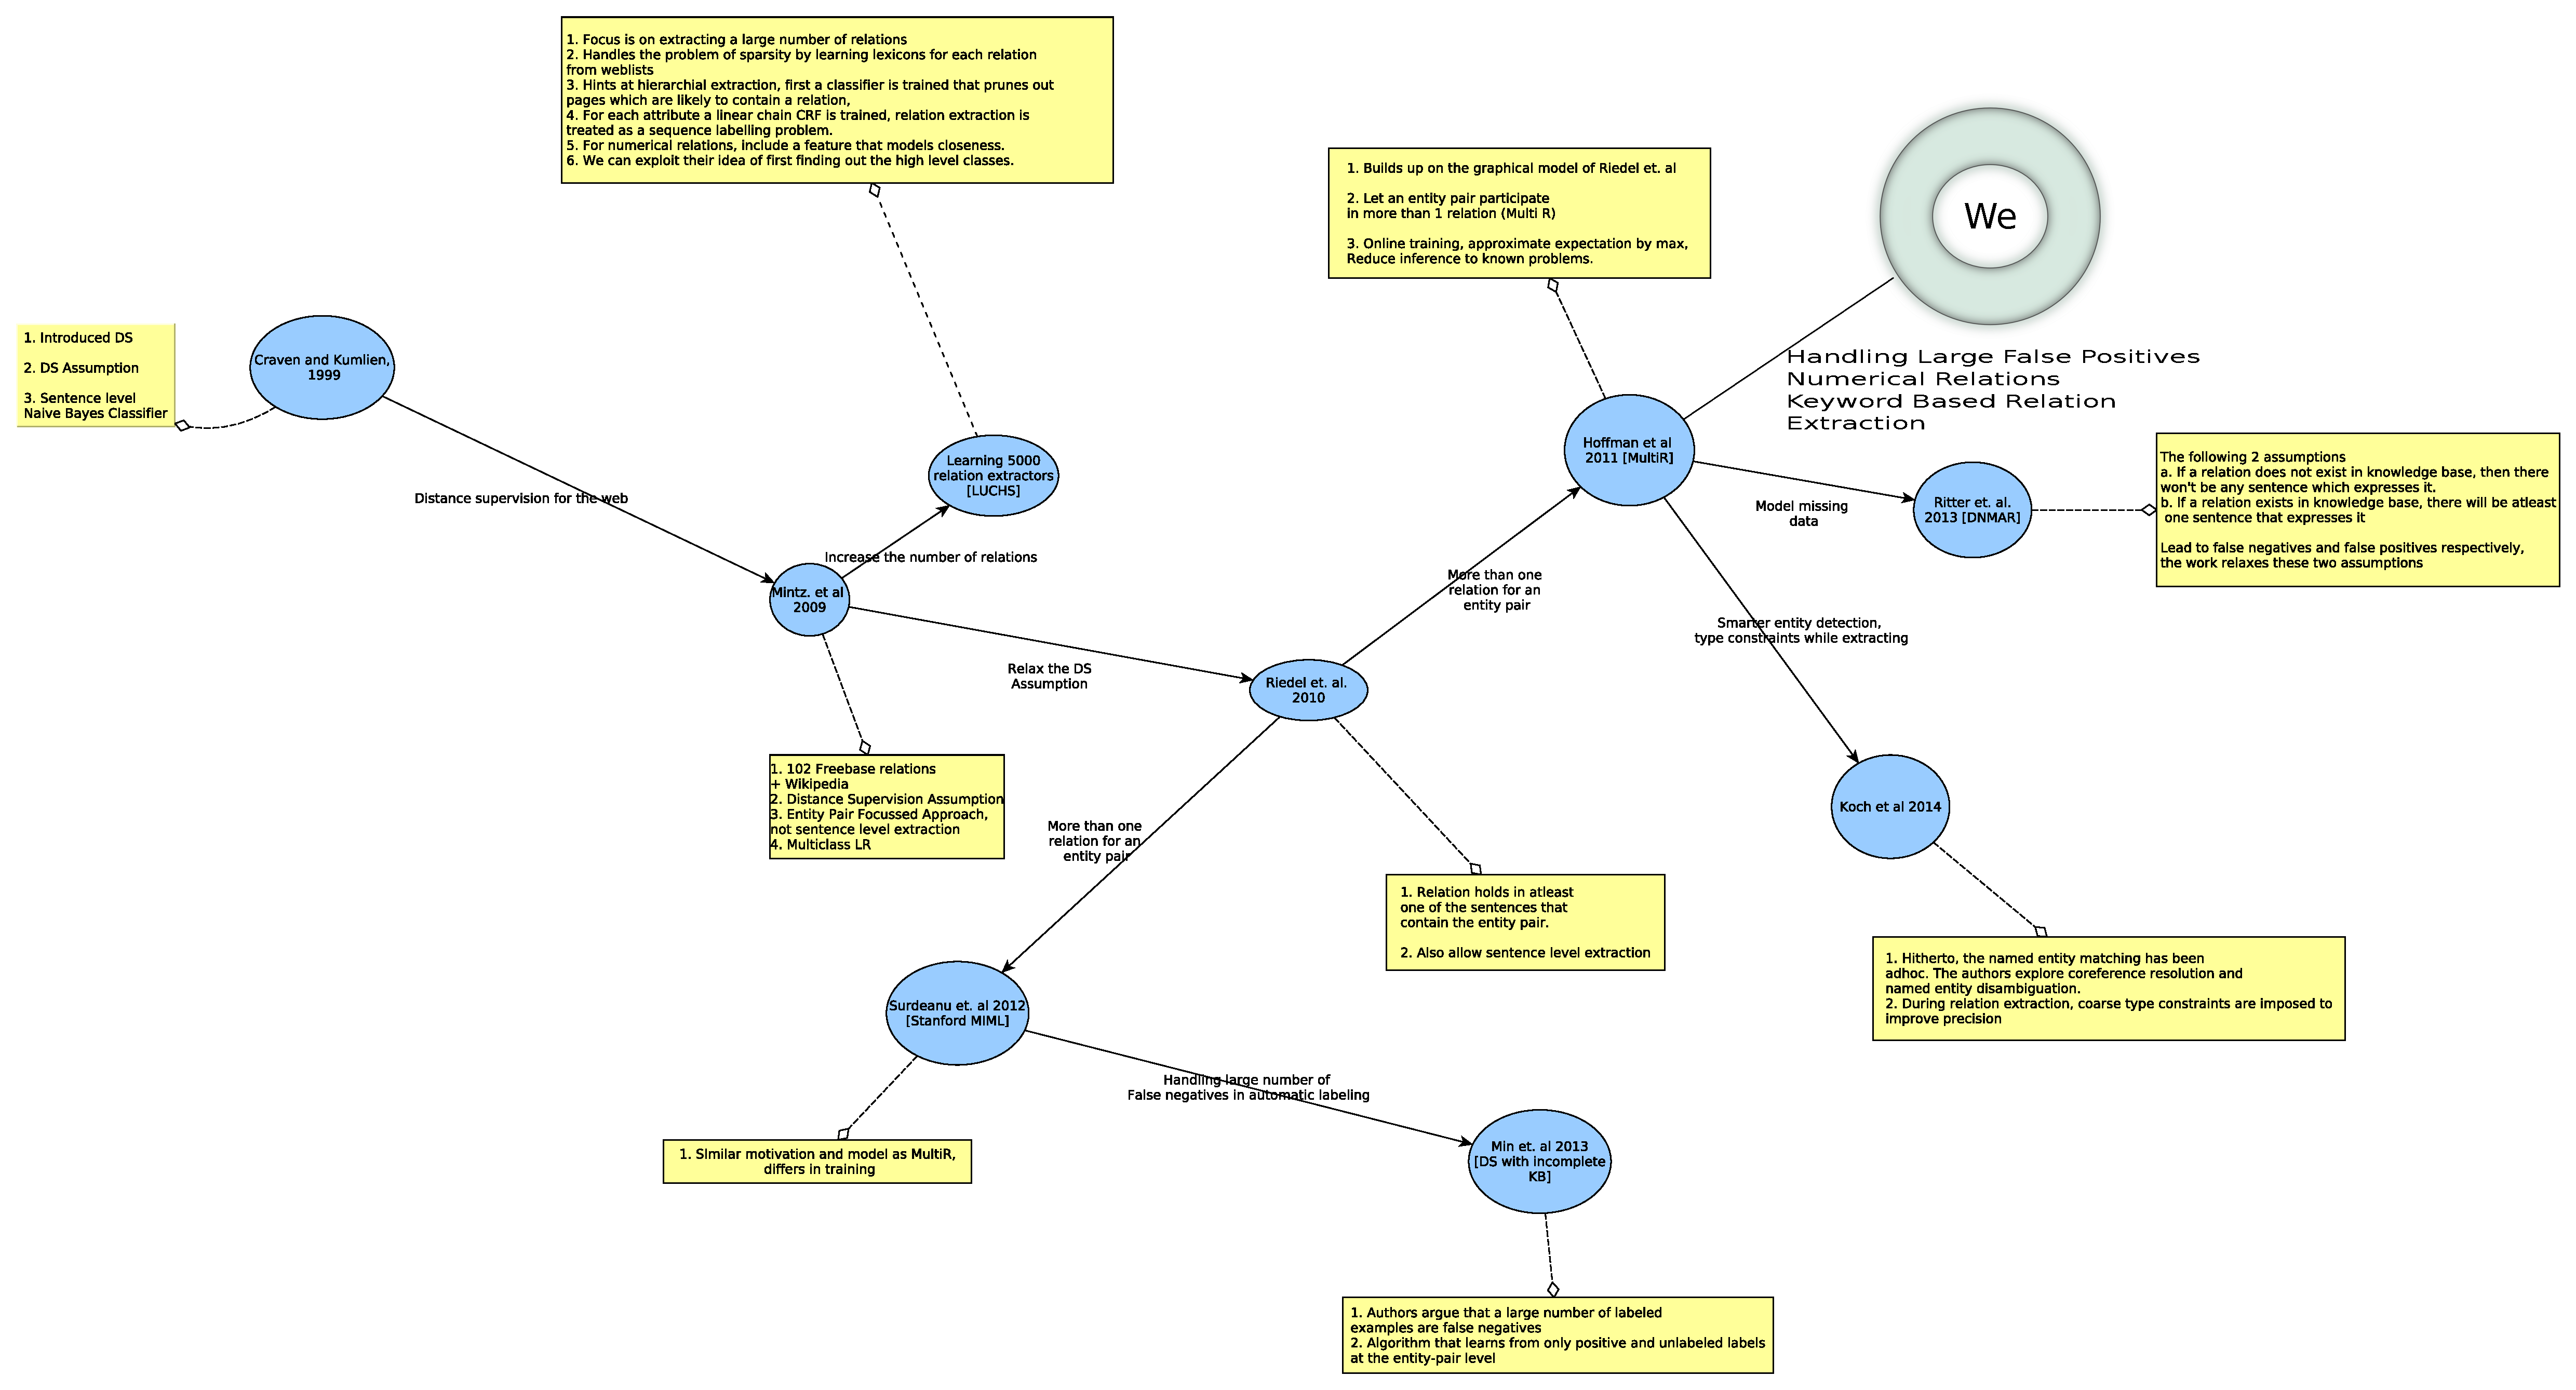
\includegraphics[scale=0.12]{./imgs/us.pdf}
 % us.pdf: 2381x1285 pixel, 72dpi, 84.00x45.33 cm, bb=0 0 2381 1285
\end{center}

\end{frame}
\section{Relation Extraction Using MultiR}
\begin{frame}{Relation Extraction Using MultiR}{From \url{raphaelhoffmann.com/publications}}
\begin{figure}[h]
 \centering
 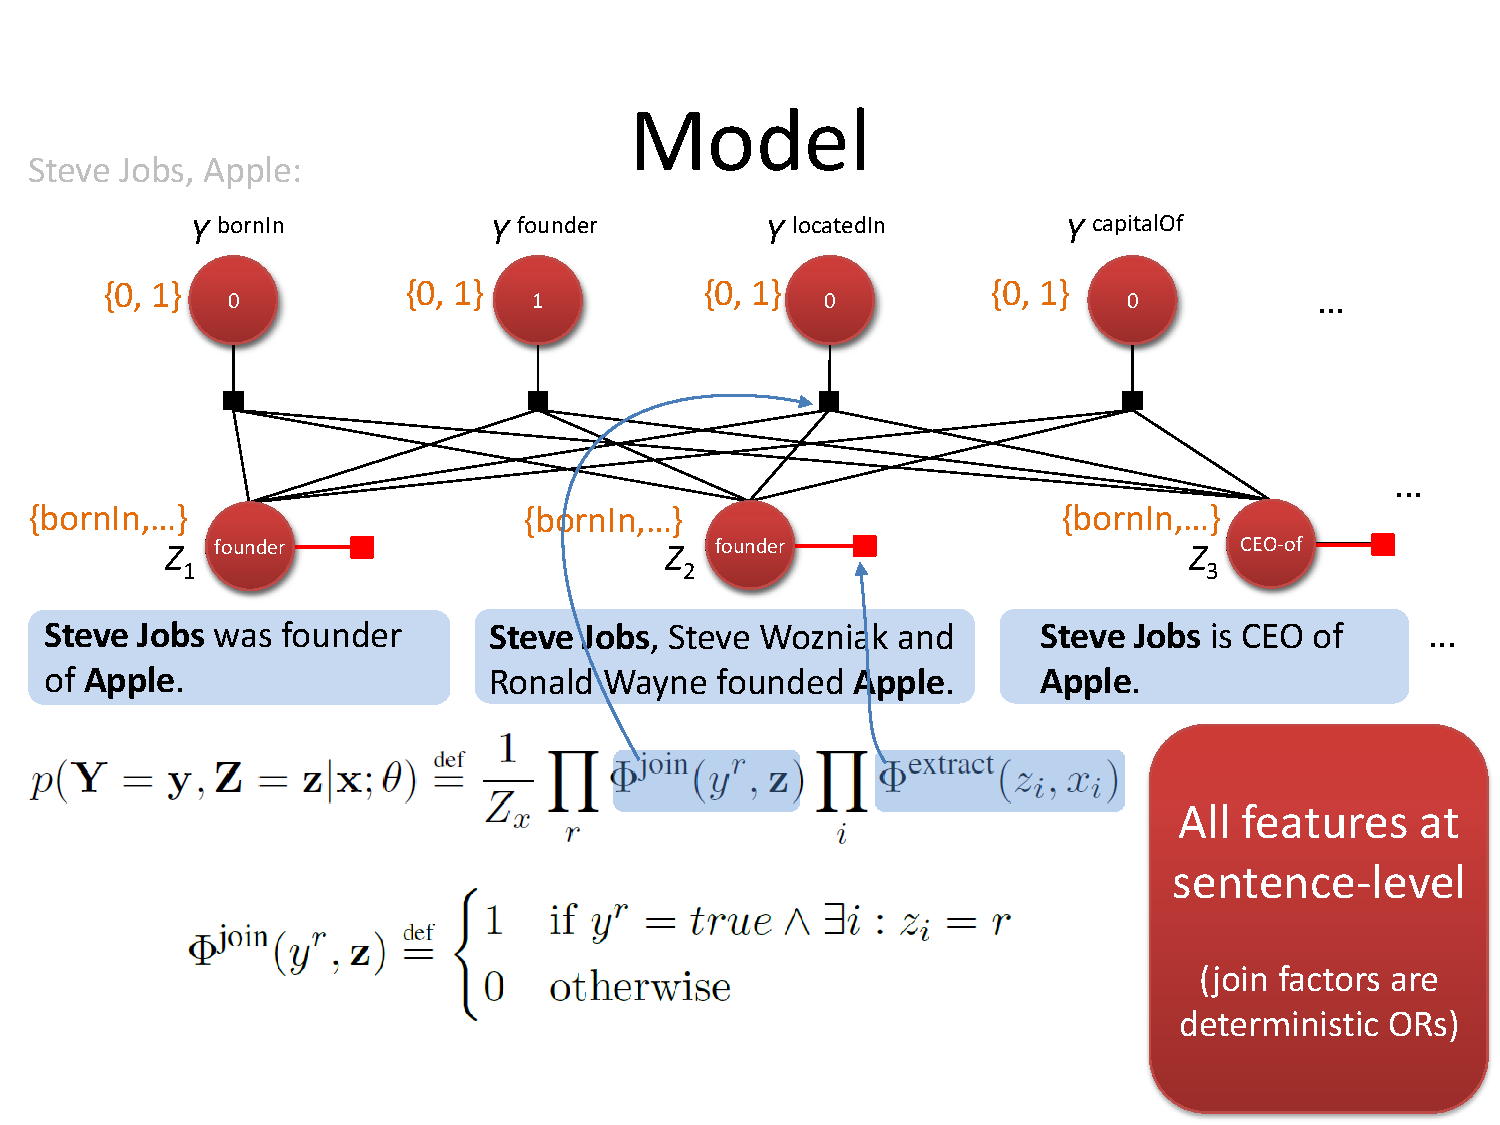
\includegraphics[scale=0.40]{./imgs/multirmode1.pdf}
 % multirmode.1.pdf: 720x540 pixel, 72dpi, 25.40x19.05 cm, bb=0 0 720 540
 \end{figure}
\end{frame}
\begin{frame}{Relation Extraction Using MultiR}{From \url{raphaelhoffmann.com/publications}}
\begin{figure}[h]
 \centering
 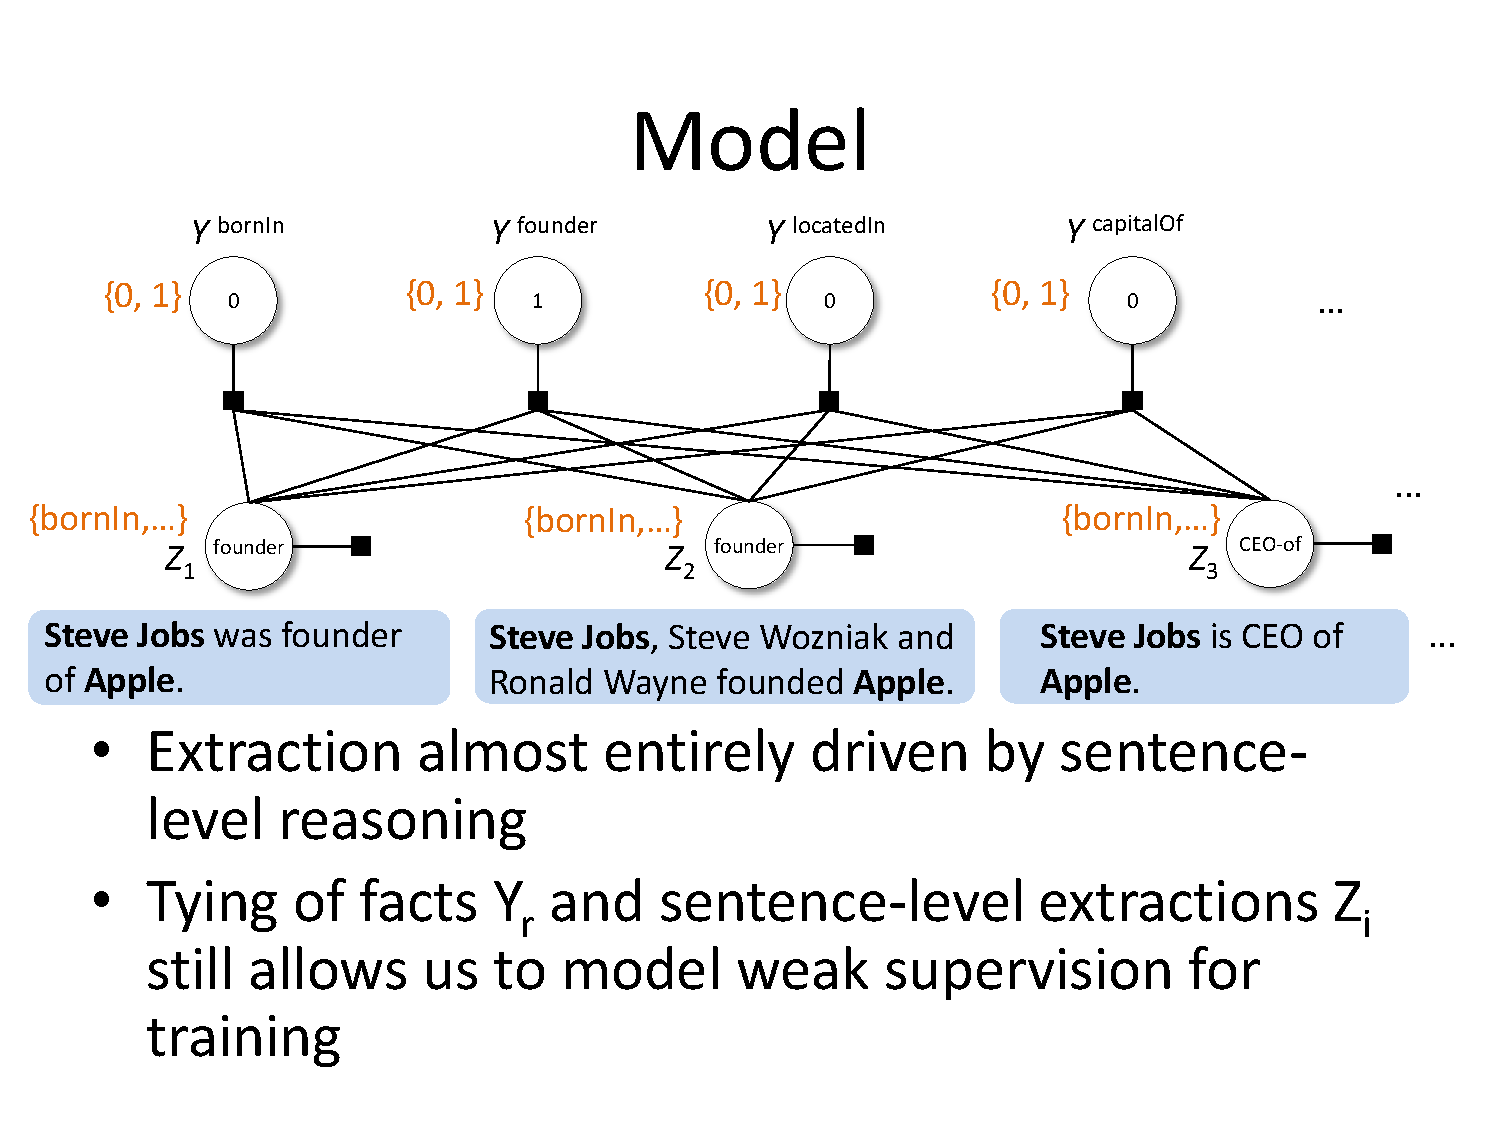
\includegraphics[scale=0.40]{./imgs/multirmode2.pdf}
 % multirmode.1.pdf: 720x540 pixel, 72dpi, 25.40x19.05 cm, bb=0 0 720 540
 \end{figure}
\end{frame}
\begin{frame}{Relation Extraction Using MultiR}{From \url{raphaelhoffmann.com/publications}}
\begin{figure}[h]
 \centering
 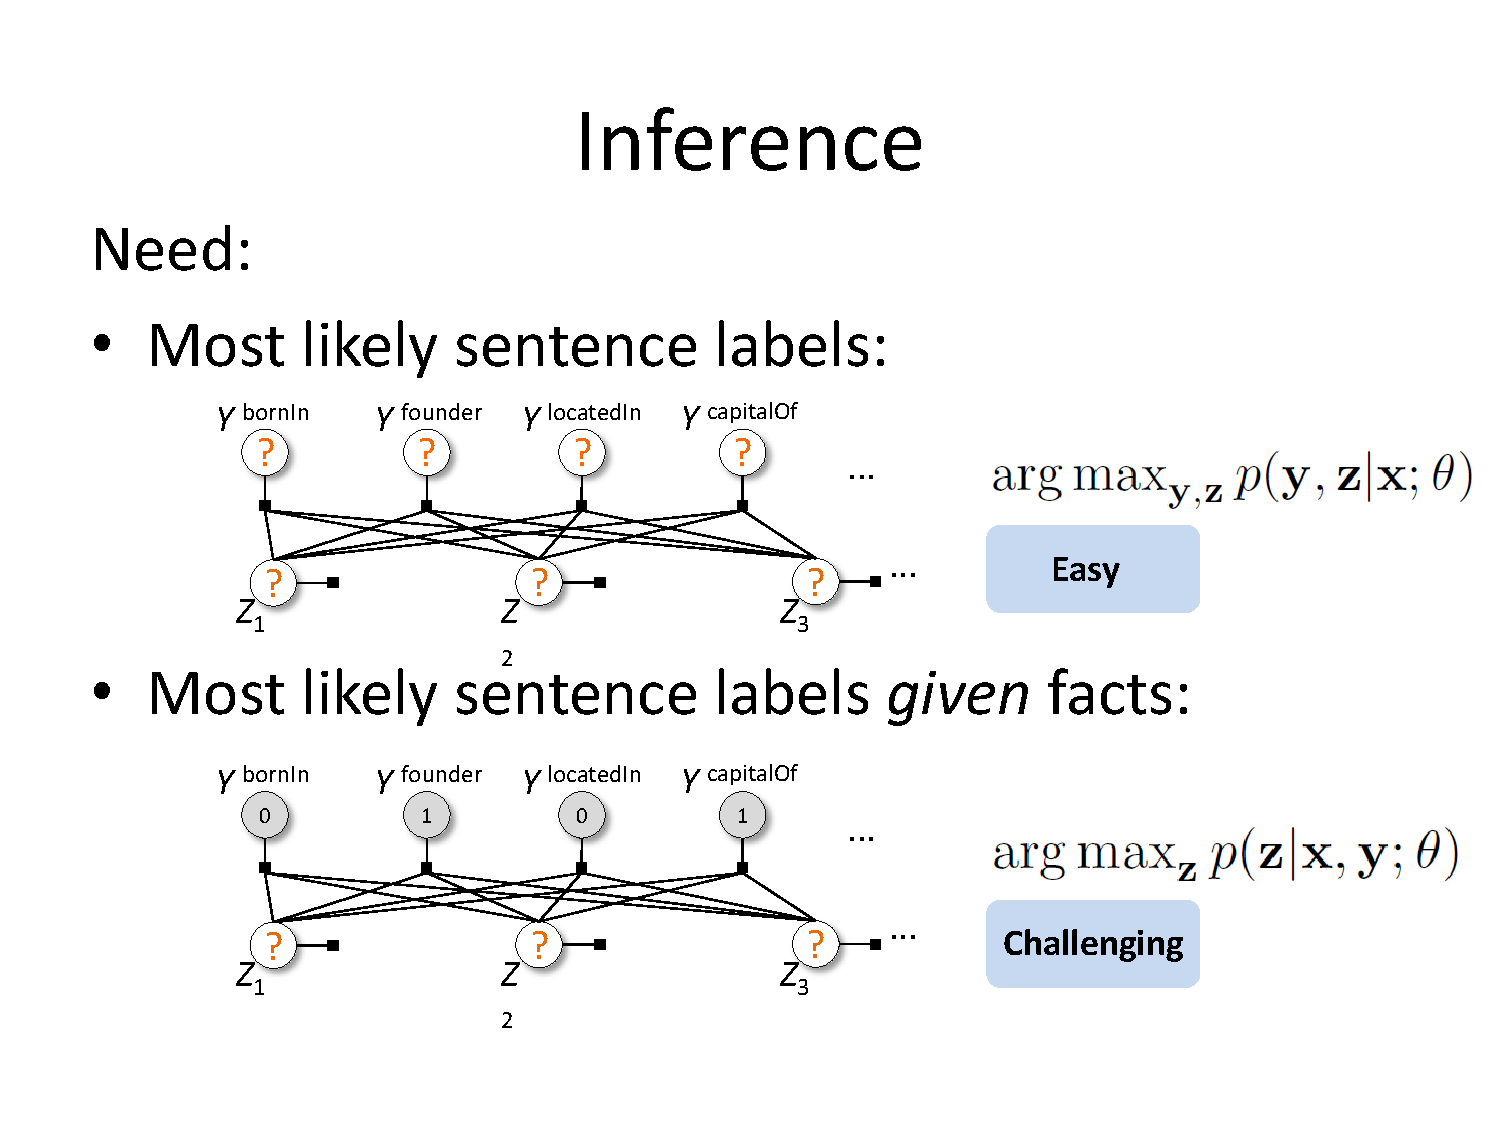
\includegraphics[scale=0.40]{./imgs/multirmode3.pdf}
 % multirmode.1.pdf: 720x540 pixel, 72dpi, 25.40x19.05 cm, bb=0 0 720 540
 \end{figure}
\end{frame}
\begin{frame}{Relation Extraction Using MultiR}{From \url{raphaelhoffmann.com/publications}}
\begin{figure}[h]
 \centering
 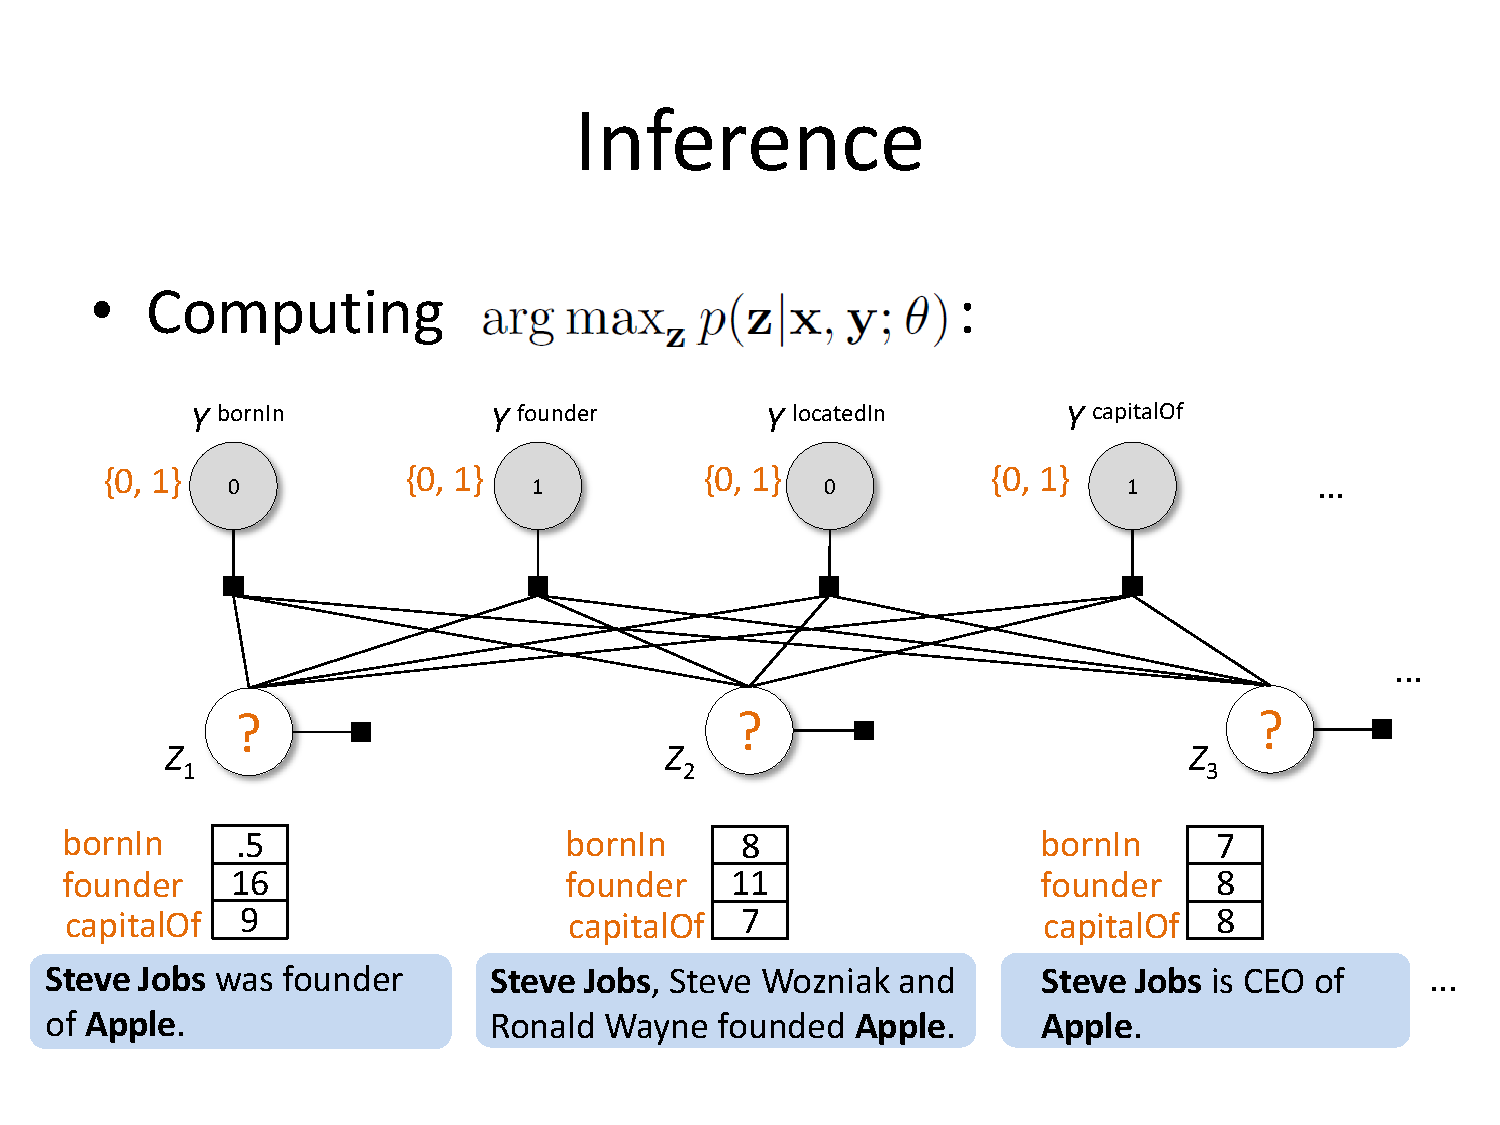
\includegraphics[scale=0.40]{./imgs/multirmode4.pdf}
 % multirmode.1.pdf: 720x540 pixel, 72dpi, 25.40x19.05 cm, bb=0 0 720 540
 \end{figure}
\end{frame}
\begin{frame}{Relation Extraction Using MultiR}{From \url{raphaelhoffmann.com/publications}}
\begin{figure}[h]
 \centering
 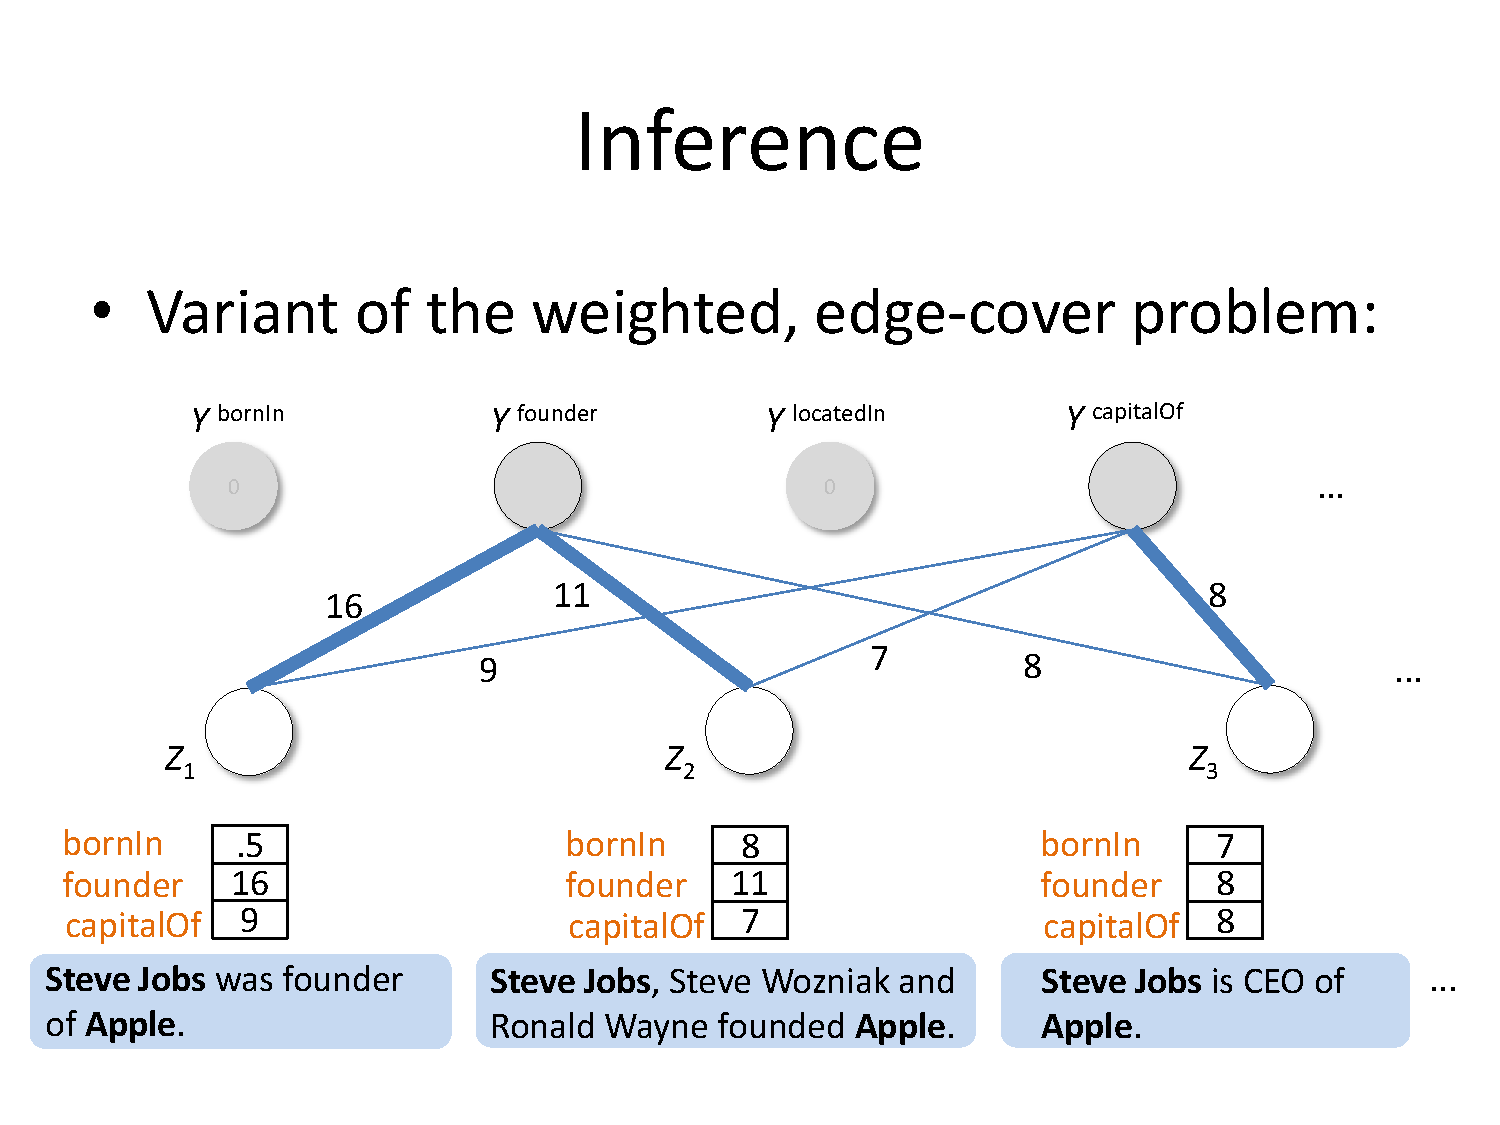
\includegraphics[scale=0.40]{./imgs/multirmode5.pdf}
 % multirmode.1.pdf: 720x540 pixel, 72dpi, 25.40x19.05 cm, bb=0 0 720 540
 \end{figure}
\end{frame}
\begin{frame}{Relation Extraction Using MultiR}{From \url{raphaelhoffmann.com/publications}}
\begin{figure}[h]
 \centering
 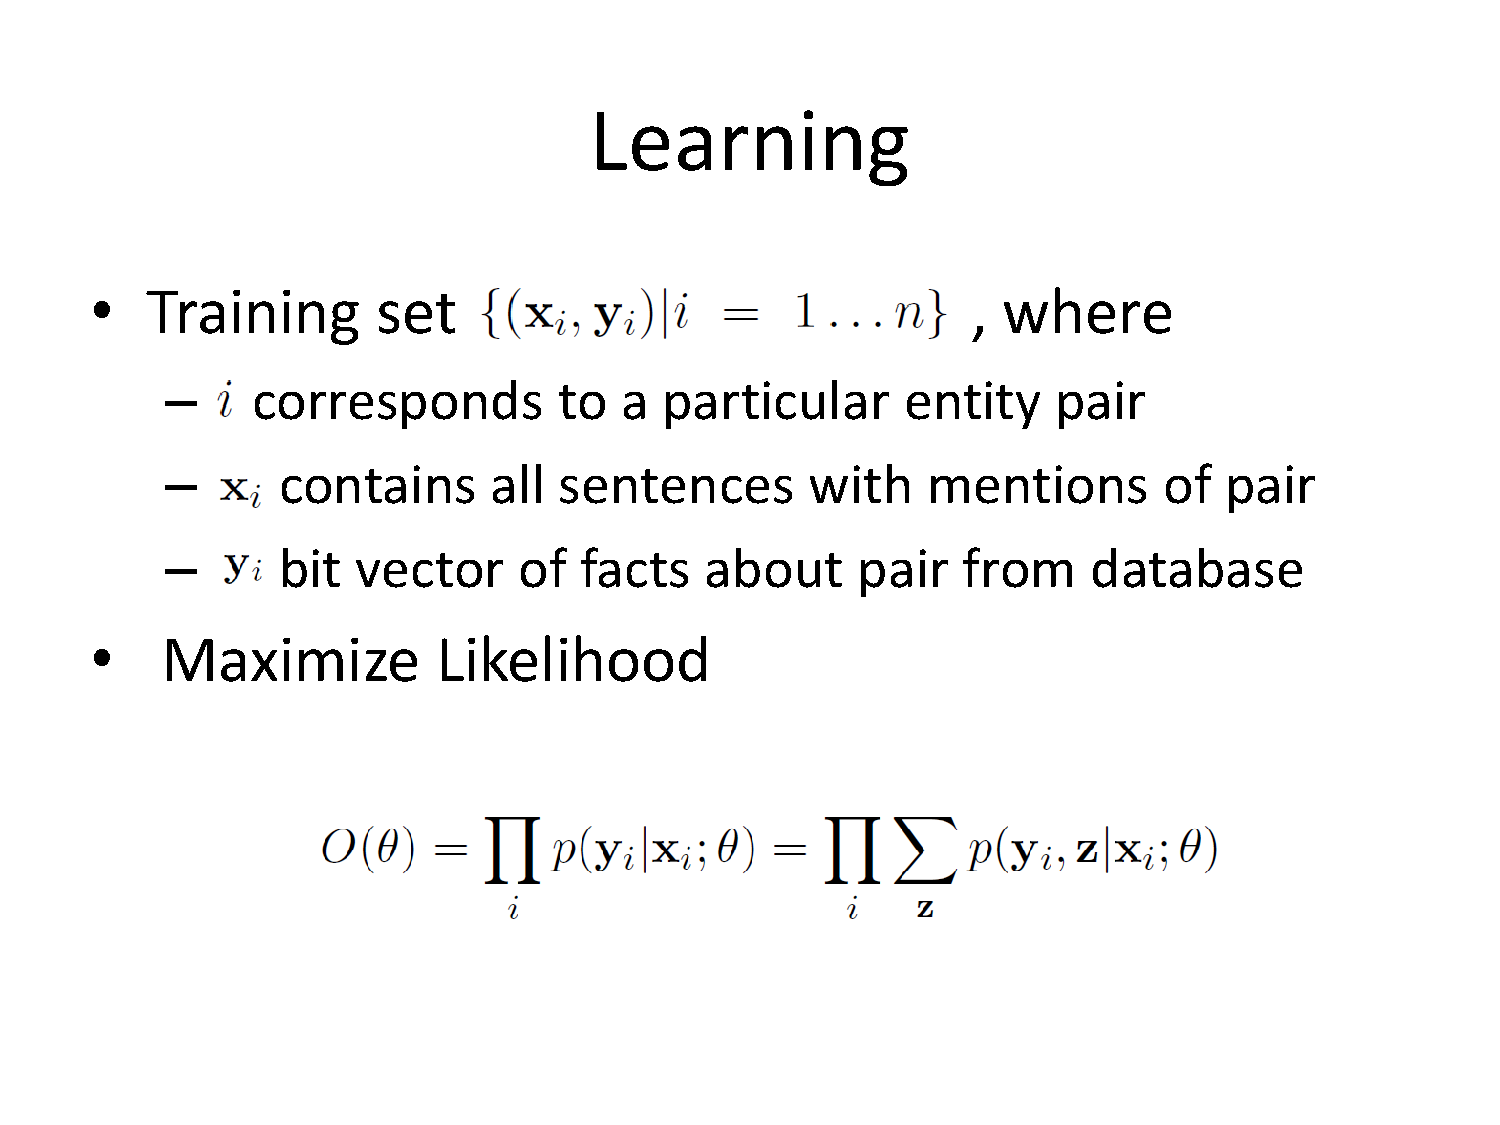
\includegraphics[scale=0.40]{./imgs/multirmode6.pdf}
 % multirmode.1.pdf: 720x540 pixel, 72dpi, 25.40x19.05 cm, bb=0 0 720 540
 \end{figure}
\end{frame}
\begin{frame}{Relation Extraction Using MultiR}{From \url{raphaelhoffmann.com/publications}}
\begin{figure}[h]
 \centering
 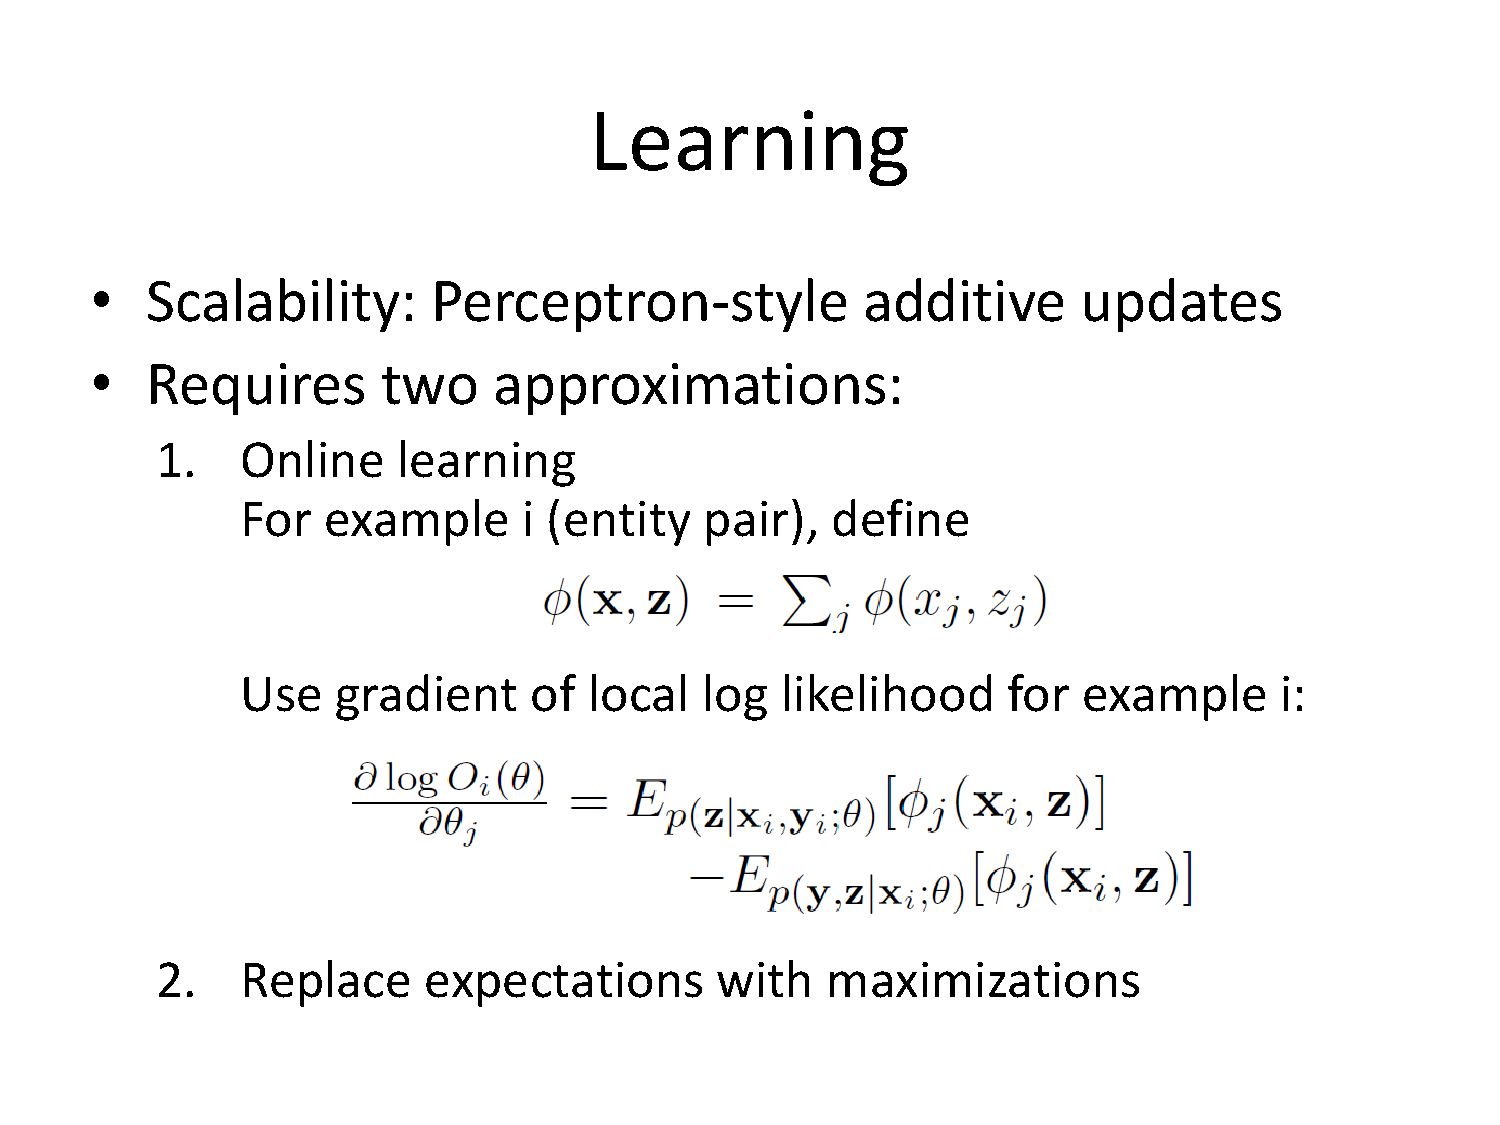
\includegraphics[scale=0.40]{./imgs/multirmode7.pdf}
 % multirmode.1.pdf: 720x540 pixel, 72dpi, 25.40x19.05 cm, bb=0 0 720 540
 \end{figure}
\end{frame}
\begin{frame}{Relation Extraction Using MultiR}{From \url{raphaelhoffmann.com/publications}}
\begin{figure}[h]
 \centering
 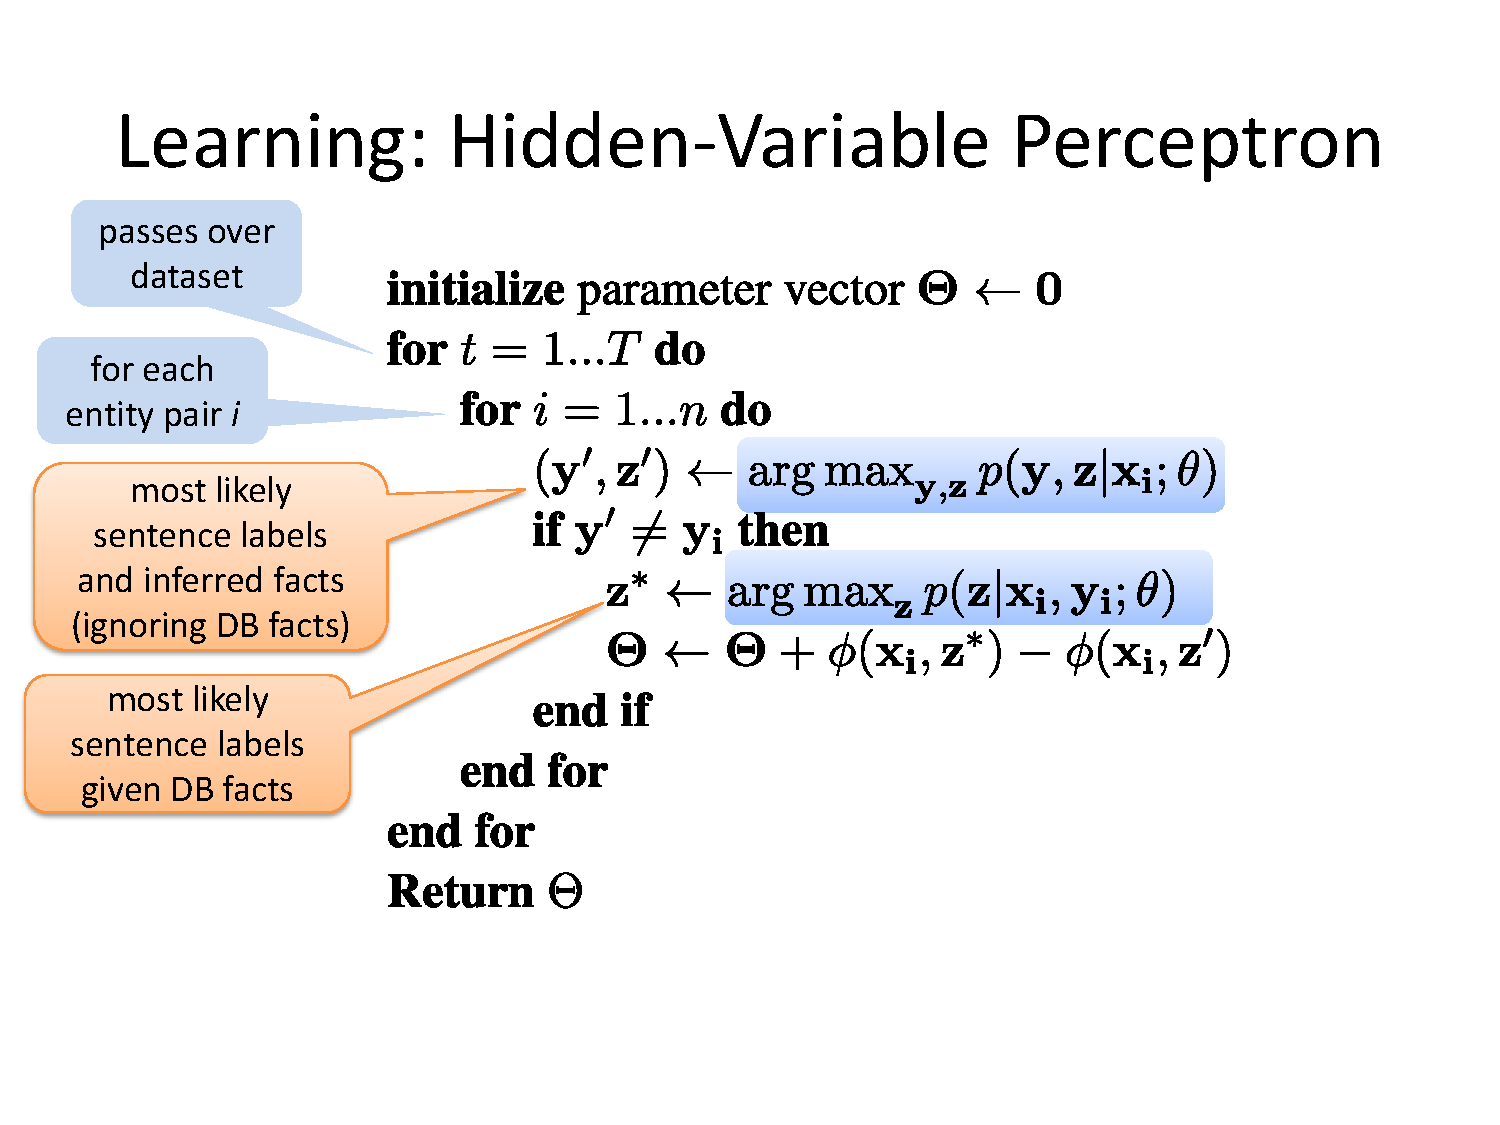
\includegraphics[scale=0.40]{./imgs/multirmode8.pdf}
 % multirmode.1.pdf: 720x540 pixel, 72dpi, 25.40x19.05 cm, bb=0 0 720 540
 \end{figure}
\end{frame}

% %PART 5: TAC Submission
\section{TAC Submission}
\begin{frame}{Cold Start Knowledge Base Population, 2014}
\begin{itemize}
\item Made a submission to Knowledge Base Population (KBP) track of TAC by tweaking the matching process to identify numbers, url's etc. as entities.\pause \\~\\
 \item Some example relations: 
    \begin{itemize}
      \item children of 
      \item city of birth  
      \item shareholders
      \item countries of residence
    \end{itemize}
  \item  Used MultiR for relation extraction\\~\\
  \item Freebase as the Knowledge base.
\end{itemize}
\end{frame}

\begin{frame}{Corpus}
 \begin{itemize}
  \item The TAC corpus consisted of three type of documents: \pause \\~\\
    \begin{itemize}
	\item \textbf{discussion forums } 99,063 English discussion forum documents selected from the BOLT Phase 1 discussion forums source data releases. Each forum includes at least 5 posts. \pause \\~\\

	\item \textbf{newswire } 1,000,257 documents selected from English Gigaword Fifth Edition. \pause \\~\\

	 \item \textbf{web} 999,999 English web documents selected from various GALE web collections. \pause \\~\\
    \end{itemize}
      
 \end{itemize}
\end{frame}


\section{Numerical Relation Extraction}
%%THIS IS PART 6 : numerical relation extraction using distant supervision




\begin{frame}{Distant supervision for Numerical Relation Extraction}{Selected Relations}
 \begin{center}
\begin{tabular}{|l|l|}
\hline
Relation Name & Relation Code \\
\hline
Land area (sq. km)&AG.LND.TOTL.K2\\
Foreign direct investment, net (current US\$)&BN.KLT.DINV.CD\\
Goods exports (current US\$)&BX.GSR.MRCH.CD\\
Electricity production (kWh)&EG.ELC.PROD.KH\\
CO2 emissions (kt)&EN.ATM.CO2E.KT\\
Pump price for diesel fuel (US\$ per liter)&EP.PMP.DESL.CD\\
Inflation, consumer prices (annual \%)&FP.CPI.TOTL.ZG\\
Internet users (per 100 people)&IT.NET.USER.P2\\
GDP (current US\$)&NY.GDP.MKTP.CD\\
Life expectancy at birth, total (years)&SP.DYN.LE00.IN\\
Population (Total)&SP.POP.TOTL\\
\hline
\end{tabular}
\end{center}

\end{frame}
\begin{frame}{Distant supervision for Numerical Relation Extraction}{Knowledge Base}
 \begin{itemize}
  \item Derived from \url{data.worldbank.org}, 4371979 numerical facts about 249 countries, 1281 attributes 
\begin{center}
\begin{tabular}{|l|l|l|}
\hline
Freebase Entity& Value & Relation\\
\hline
/m/04g5k&3126000130&Electricity Production\\
/m/02k8k&1969.179&$CO_{2}$ Emission\\
/m/06nnj&332315&Total Population\\
/m/019rg5&55.020073&Life Expectancy\\
/m/05sb1&19974.148&$CO_{2}$ Emission\\
/m/05v8c&10000000000&Electricity Production\\
/m/03spz&7639000100&Electricity Production\\
/m/06vbd&44249.688&$CO_{2}$ Emission\\
/m/0d060g&51.3&Internet Users(\%)\\
/m/05qkp&62.298927&Life Expectancy\\
\hline
\end{tabular}
\end{center}

\end{itemize}

\end{frame}

\begin{frame}{Distant supervision for Numerical Relation Extraction}{Corpus}

\begin{itemize}
 \item Subset of the tac corpus \\~\\
 \item 268, 036 Documents,  sentences having a country and a number  \\~\\
 \item List of countries augmented manually by adding all possible synonyms (Dutch, Netherlands) and inflections (Ireland, Irish)
\end{itemize}
\end{frame}

\begin{frame}{Distant supervision process for numerical relation extraction}{Preprocessing}
 \begin{figure}[h]
 \centering
 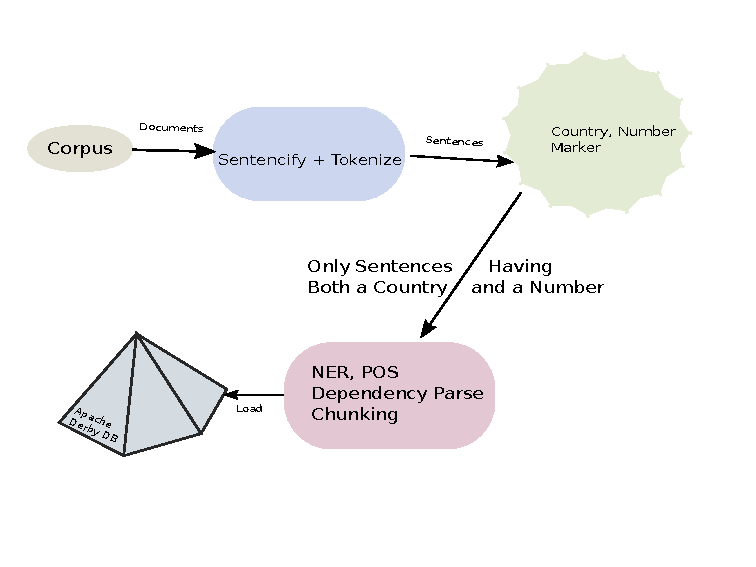
\includegraphics[bb=0 0 363 272, scale = 0.8]{./imgs/pipeline.pdf}
 % pipeline.pdf: 363x272 pixel, 72dpi, 12.81x9.60 cm, bb=0 0 363 272
\end{figure}
\end{frame}

\begin{frame}{Distant supervision process for numerical relation extraction}{Handling the Scale}
 
\begin{itemize}
 \item Hadoop based NLP pipeline {\tiny \url{https://github.com/NEO-IE/Hadoop-Scripts}}
 \item Used portions of: {\tiny \url{https://github.com/jgilme1/CorpusProcessing-Hadoop-Multir}}
\end{itemize}

\begin{figure}[h]
 \centering
 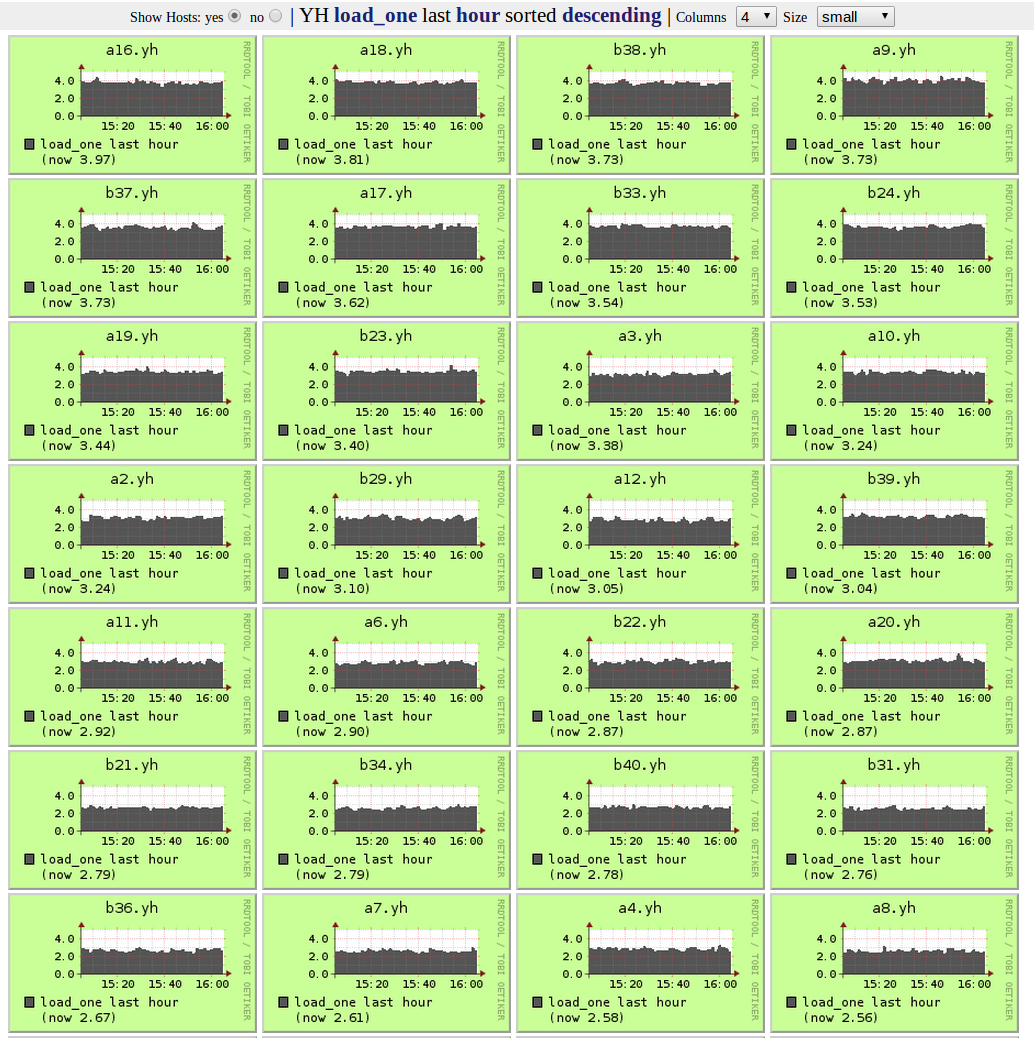
\includegraphics[bb=0 0 1680 1050,scale=0.2]{./imgs/clusterworking.png}
 % clusterworking.png: 1680x1050 pixel, 72dpi, 59.27x37.04 cm, bb=0 0 1680 1050
\end{figure}

\end{frame}


\begin{frame}{Distant supervision process for numerical relation extraction}
 \begin{itemize}
  \item Extract a country and number from a sentence, go to kb and check if there is a match. \\~\\
  \item Can be creative during matching: \\~\\
  \begin{itemize} 
   \item Distance based matching \\~\\
   \item Time based matching 
  \end{itemize}
 \end{itemize}
\end{frame}

\begin{frame}{First Attempt: Vanilla Matching}
 \begin{center}
 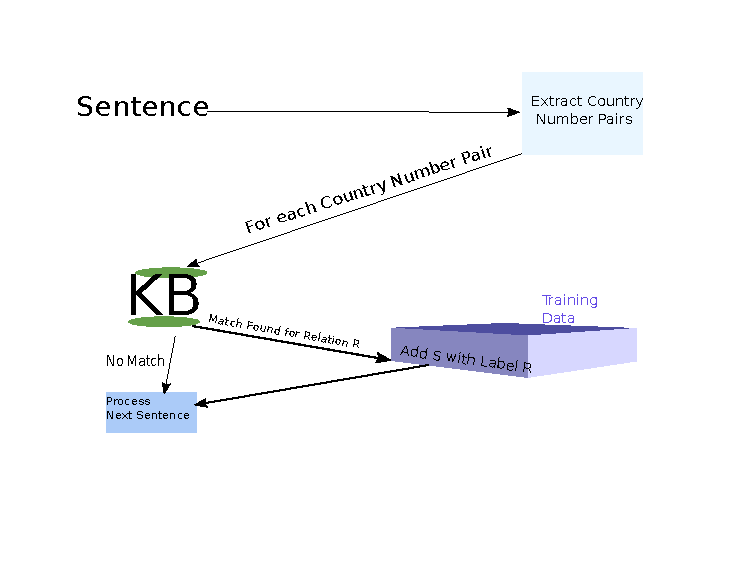
\includegraphics{./imgs/simple.pdf}
 % simple.pdf: 363x272 pixel, 72dpi, 12.81x9.60 cm, bb=0 0 363 272
\end{center}
\end{frame}
%TODO : Add distribution of matches per relation

\begin{frame}{Vanilla Matching: Results}
\begin{center}
 \resizebox{\linewidth}{!}{% Resize table to fit within \linewidth horizontally
 
\begin{tabular}{|l|l|l|l|l|}
\hline
Relation&Total Matches&Sampled Matches&True Matches&Precision(\%)\\
\hline
Land Area&1884&15&\textbf{1}&\textbf{6.7}\\
Foreign Direct Investment&0&0&0&0\\
Goods Export&0&0&0&0\\
Electricity Production&381&10&0&0\\
$CO_{2}$ Emission&0&0&0&0\\
Diesel Prices&8491&15&0&0\\
Inflation(\%)&8689&15&0&0\\
Internet Users(\%)&182319&40&0&0\\
GDP(\$)&0&0&0&0\\
Life Expectancy&267&10&0&0\\
Total Population&0&0&0&0\\
\hline
\end{tabular}}
\end{center}
 \begin{itemize}
  \item A large number of matches \smiley
  \item Most of them false positives  \frownie
 \end{itemize}

\end{frame}

\begin{frame}{Sample Matches for Vanilla Matching}{False Positives}

 \begin{table}
 \tiny
 \centering
 \begin{tabularx}{\textwidth}{|l|l|l|>{\raggedright}X|}
 \hline
 \textbf{Country} & \textbf{Relation} & \textbf{Value} & \textbf{Sentence}\tabularnewline
 \hline
  South Africa & Internet Users(\%) & 24 & Montjane, \textbf{24}, was crowned on Sunday evening at the Superbowl at Sun City, in \textbf{South Africa}'s North  West province.\tabularnewline
  \hline
 Croatia & Inflation & 500 & \textbf{Croatian} police say more than \textbf{500} guns turned in after the country's 1991 war were stolen from a police depot and sold on the black market.\tabularnewline
  \hline
  France & Life Expectancy & 75 & \textbf{France}: Hugo Lloris, Eric Abidal, Patrice Evra, William Gallas, Bacary Sagna, Abou Diaby, Yoann Gourcuff (Florent Malouda, \textbf{75}), Jeremy Toulalan, Nicolas Anelka (Thierry Henry, 72), Sidney Govou (Andre-Pierre Gignac, 85), Franck Ribery.\tabularnewline
  \hline
  France & Diesel prices & 1.72 & Lotte Friis of Denmark won the women's 800 freestyle in 8:23.27, followed at 0.73 seconds by Ophelie Cyriell Etienne of \textbf{France} and Federica Pellegrini of Italy, \textbf{1.72} seconds back.\tabularnewline
  \hline
  Bermuda & Land Area(sq. km) & 50 & Forecasters were also closely tracking the path of Tropical Storm Fiona about 360 miles (580 km) south of \textbf{Bermuda}, with wind speeds of up to \textbf{50} miles (85 km) per hour.\tabularnewline
  \hline
 \end{tabularx}
 \end{table}
 \end{frame}
 
 \begin{frame}{Key Observations on vanilla matching}
  
  \begin{itemize}
   
   \item Units for \textbf{precision}, not just recall. \\~\\
   
   \item \textbf{Dates} and \textbf{Sports} articles lead to a lot of false positives. \\~\\
   
   \item \textbf{Small numbers} generate larger false positives; finer numbers generate fewer false positives. \\~\\
    \begin{itemize}
      \item Intuitively, it makes sense that we'll see a lot of 2s, 3s, 71s in different contexts than 1,000,232,112. 
      \item Getting an exact match for 23.14152 is more difficult than matching 23. \\~\\
    \end{itemize}
  \end{itemize}
 \end{frame}



\begin{frame}{False Positives}{Numbers are weak entities}
\begin{itemize}
 \item Vanilla numerical relation matching is \textbf{bound} to attract humongous amounts of false positives; \pause \\~\\
 \item Stems from the fact that \emph{numbers don't have an identity of their own}. \pause \\~\\
 \item Consider {\SoulColor\hl{India}} and {\SoulColor\hl{Mumbai}} Vs. {\SoulColor\hl{India}} and {\SoulColor\hl{19}} \pause \\~\\
 \item {\SoulColor\hl{Mumbai}} is a strong entity, {\SoulColor\hl{19}} is a \textbf{weak} entity. 
 \end{itemize}
\end{frame}
\begin{frame}{False Positives}{Numbers are weak entities}
 \begin{itemize}  
 \item Number of sentences in which {\SoulColor\hl{India}} and {\SoulColor\hl{Mumbai}} appear together, vs the number of sentences
  in which {\SoulColor\hl{India}} and {\SoulColor\hl{19}} appear together. \pause \\~\\
 \item Just {\SoulColor\hl{19}} can be appear with India in several contexts: \pause \\~\\
 \begin{itemize} 
 \item Internet user \% \pause 
 \item Billion dollars invested by a company \pause 
 \item \% of people below the poverty line \pause 
 \item date (if we are not careful) \pause 
 \item number of medals won by Indian athletes... \pause \\~\\
\end{itemize} 

 \item Can we expect the situation to be even worse for certain types of numbers?
\end{itemize}
\end{frame}
%PART 7 : Units
\section{The role of Units}
\begin{frame}{Numbers are Incomplete without Units} \pause
 
 \begin{itemize}
  
  \item  Attributes represented by numbers usually have associated units \pause
  \begin{figure}[h]
 \centering
 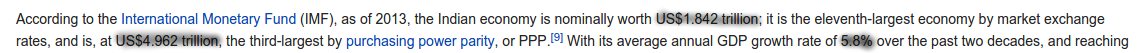
\includegraphics[bb=0 0 1139 53,scale=0.27]{./images/ex_6.png}
 % ex_6.png: 1139x53 pixel, 72dpi, 40.18x1.87 cm, bb=0 0 1139 53
\end{figure}

  \pause 
  \item Units help in \textbf{improving recall.}  \pause \\~\\ 
  
  \begin{itemize}
      \item In above example 1.842 as number alone would not match with the fact regarding economy in knowledge base. \pause \\~\\
      \item But with the unit trillion USD, we can normalize the value and then it would match existing facts in knowledge base. 
      
  \end{itemize}
  \end{itemize}
  \end{frame}

\begin{frame}{Numbers are Incomplete without Units} 
    \begin{figure}
    \centering
    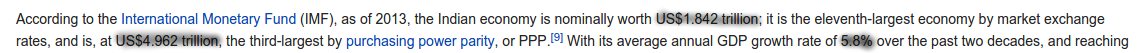
\includegraphics[width = 1.0\textwidth]{images/ex_6}
  \end{figure}
  
  \begin{itemize}
  \item Units help in reducing false positives and hence \textbf{improving precision.} \pause \\~\\
  \begin{itemize}
      \item If there is a fact, e.g, \textbf{inflation(India, 1.842\%)} in knowledge base, then ignoring units can cause an incorrect match which leads in learning towards noisy patterns. \\~\\
  \end{itemize}
  
 \end{itemize}

 
\end{frame}

\begin{frame}{Unit Extraction is not easy!} \pause
 
 \begin{itemize}
    \item Different ways to represent a single unit. \pause 
    \begin{itemize}
     \item Tunisia occupies an area of 163,610 \textbf{square kilometres}, of which 8,250 are water. \pause \\~\\
     \item With an area of about 9.6 \textbf{million $km^{2}$}, the People's Republic of China is the 3rd largest country in total area behind Russia and Canada, and very similar to the United States. \\~\\
    \end{itemize}
\pause
    \item Multiple units to represent a single numerical fact. \pause
    \begin{itemize}
      \item Vatican City, a walled enclave within the city of Rome, with an area of approximately \textbf{44 hectares} \textbf{(110 acres)}, and a population of 842, is the smallest internationally recognized independent state in the world by both area and population. \\~\\
    \end{itemize}
 \item We use unit tagger \url{https://github.com/ssprojects/UnitTagger} by Prof. Sunita Sarawagi
 \end{itemize}
 
\end{frame}


\begin{frame}{Overview of Unit Extraction System} \pause
 
 \begin{itemize}
  
  \item A discriminative context free grammmar with scores
attached to each possible production in the grammar. \pause \\~\\ 
  \item A production P in the grammar is of the form  $ R ::= R_{1} R_{2}$ , scored as 
\begin{equation*}
	score(P) = \textbf{w . f}(P, x, i, j, k), 
\end{equation*}
where $(i,j)$ and $(j+1,k)$ are text spans in $x$ that $R_{1}$ and $R_{2}$
cover.
 \end{itemize}
\end{frame}

\begin{frame}{Overview of Unit Extraction System}
 \begin{itemize}
  \item Some of the features that grammar uses to assign the best scores to various 
parses are as belows: \pause \\~\\
    \begin{itemize}
        \item Matches with Unit Catalog \pause \\~\\
	\item Lexical Clues \pause \\~\\
	\item Relative Frequency - Prior of the word to be present as unit, then as an
	  non-unit word. This is derived from WordNet ontologies. \pause \\~\\
	\item Co-occurrence statistics - presence of strongly co-occuring words in the
	  text can help in disambiguating the various candidate units 
    \end{itemize}
 \end{itemize}
 
\end{frame}

\begin{frame}{Units Based Matching: Results}
\begin{center}
 \resizebox{\linewidth}{!}{% Resize table to fit within \linewidth horizontally
 
\begin{tabular}{|l|l|l|l|l|}
\hline
Relation&Total Matches&Sampled Matches&True Matches&Precision(\%)\\
\hline
\textbf{Land Area} &98	& 40 & 32 &80\\
Foreign Direct Investment & 791 & 40& 1&2.5\\
Goods Export&816&40&3&7.5\\
Electricity Production&19&19&0&0\\
$CO_{2}$ Emission&196&40&2&5\\
Diesel Prices&2&2&2&100\\
Inflation(\%)&27598&40&0&0\\
Internet Users(\%)&24639&40&0&0\\
GDP(\$)&1790&40&0&0\\
Life Expectancy&3081&40&0&0\\
\textbf{Total Population}&5225&40&11&27.5\\
\hline
\end{tabular}}
\end{center}

\end{frame}

\begin{frame}{Sample Matches for Unit Based Matching}


 \begin{table}
 \centering
 \tiny
 \begin{tabularx}{\textwidth}{|l|l|l|>{\raggedright}X|}
 \hline
 \textbf{Country} & \textbf{Relation} & \textbf{Value} & \textbf{Sentence}\tabularnewline
 \hline
 Lebanon & Land Area & $1.02 x 10^{11}$ sq m & \textbf{Lebanon} lies in the eastern Mediterranean and covers about \textbf{4,030 square miles} (10,450 square kilometers) -- smaller than the U.S. state of Connecticut.\tabularnewline
  \hline
  Russia & Goods Export & $ 10^{10}$ USD & The IMF agrees to offer a loan of \textbf{US\$10.2 billion} to \textbf{Russia} over the next three years to help Russians transform their economy.\tabularnewline
  \hline
  Australia & Internet Users(\%) & 0.6\% & South Korea's main index added \textbf{0.6 percent}, China's Shanghai's benchmark climbed 1.5 percent and \textbf{Australia}'s index advanced 1.1 percent.\tabularnewline
  \hline
  Israel & Internet Users(\%) & 20.0\% & \textbf{Israel}'s Arab community numbers 1.3 million, about \textbf{20 percent} of the population.\tabularnewline
  \hline
  Pakistan & Life Expectancy(years) & 60 & Why does a small elite still control vast swaths of land more than \textbf{60 years} after \textbf{Pakistan} became a nation?\tabularnewline
  \hline
 \end{tabularx}
 \end{table}
 \begin{itemize}
 \item Better, but just units are not enough for most of the cases. 
  \item \% still attracts false positives
 \end{itemize}

 \end{frame}

\begin{frame}{Key Observations on Unit Based Matching}
 
 \begin{itemize}
  \item Attributes with Unit \% (inflation, internet user \%), are affected by stock data that is heavily present in the news corpus.\\~\\
  \item Almost similar values for relations FDI, Goods Export, GDP.\\~\\
  \item An (entity, number) pair matches all of the three relations. \\~\\
  \item Indicates that we might need some relation specific heuristics. \\~\\
 \end{itemize}

 
\end{frame}


%PART 8 : Keywords
\section{Keywords}
\begin{frame}{A case for Keywords}
 \begin{itemize}
  \item A large number of false matches had no reference to the relation involved.
  \item Eg. \textbf{No mention of Population} in the following matches:
  \begin{itemize}
  \item The website of \SoulColor\hl{China's} Ministry of Defense (MOD) has attracted around \SoulColor\hl{1.25} billion visits in the three months since its opening, with the United States topping the source countries for foreign visits, website editor-in-chief Ji Guilin said.
  \item Insulza, for his part, said the Organization of American States expects to raise \SoulColor\hl{10 million} dollars for \SoulColor\hl{Haiti's} recovery.
  \item Koloini and others brought 10 million euros, probably \SoulColor\hl{15 million}, back from \SoulColor\hl{Iraq} at the time, Falter quoted from the diary.
 \end{itemize}
\item \textbf{No reference to Co2 emission}:
 \begin{itemize}
 \item \SoulColor\hl{China's} iron ore imports surged 41.6 percent to \SoulColor\hl{627.8 million tonnes} in 2009, with the value falling 17.4 percent as prices were hit by the global downturn, customs data shows.
 \end{itemize}
 \end{itemize}
\end{frame}

\begin{frame}{A case for Keywords}
 \begin{itemize}
  \item A large number of false matches had no reference to the relation involved.
  \item Eg. \textbf{No mention of Population} in the following matches:
  \begin{itemize}
  \item The website of \SoulColor\hl{China's} Ministry of Defense (MOD) has attracted around \SoulColor\hl{1.25} billion visits in the three months since its opening, with the United States topping the source countries for foreign visits, website editor-in-chief Ji Guilin said. {\color{red} Will Match!}
  \item Insulza, for his part, said the Organization of American States expects to raise \SoulColor\hl{10 million} dollars for \SoulColor\hl{Haiti's} recovery. {\color{red} Will Match!}
  \item Koloini and others brought 10 million euros, probably \SoulColor\hl{15 million}, back from \SoulColor\hl{Iraq} at the time, Falter quoted from the diary. {\color{red} Will Match!}
 \end{itemize}
\item \textbf{No reference to Co2 emission}:
 \begin{itemize}
 \item \SoulColor\hl{China's} iron ore imports surged 41.6 percent to \SoulColor\hl{627.8 million tonnes} in 2009, with the value falling 17.4 percent as prices were hit by the global downturn, customs data shows. {\color{red} Will Match!}
 \end{itemize}
 \end{itemize}
\end{frame}

\begin{frame}{A case for Keywords}
 \begin{exampleblock}{Good News}
  Sentences expressing a numerical relation can be expected to have keywords that denote the relation
 \end{exampleblock}

 \begin{itemize}
  \item Take all the labeled sentences, prune out sentences that don't have at least one of the relevant keywords.
 \end{itemize}
 \begin{table}
  \tiny

 \begin{tabular}{|l|l|}
  \hline
  Internet User \% & "Internet" \\
Land Area & "area", "land", "land area" \\
Population &"Population" \\
Diesel & "diesel" \\
GDP &"Gross domestic", "GDP" \\
CO2 &"Carbon", "Carbon Emission", "CO2" \\
Inflation & "Inflation", "Price Rise" \\
FDI & "Foreign", "FDI" \\
Goods Export & "goods" \\
Life Expectancy & "life", "life expectancy" \\
Electricity Production & "Electricity" \\
 \hline
 \end{tabular}
 \end{table}
\end{frame}
\begin{frame}{A case for Keywords}
\begin{itemize} 
  \item Numbers are the second entity in our setup (Relation(Country, Number)) \\~\\
  \item Unlike real world entities, numbers don't have an identity of their own, sentences should have words (keywords!) indicating what the number stands for \\~\\
  \item Manual inspection of 400 sentences pruned out after applying keyword based filter backs this conjecture, \textbf{not even one} false negative \\~\\
  \item The keywords are created manually, can this process be automated?
\end{itemize}
\end{frame}
\begin{frame}{Keywords + Units Based Matching: Results}
\begin{center}
 \resizebox{\linewidth}{!}{% Resize table to fit within \linewidth horizontally
 
\begin{tabular}{|l|l|l|l|l|}
\hline
Relation&Total Matches&Sampled Matches&True Matches&Precision(\%)\\
\hline
\textbf{Land Area}&61&40&\textbf{30}&\textbf{75}\\
Foreign Direct Investment&8&0&0&0\\
Goods Export&4&4&0&0\\
Electricity Production&0&0&0&0\\
$CO_{2}$ Emission&16&16&2&12.5\\
Diesel Prices&2&2&2&100\\
\textbf{Inflation(\%)}&3853&40&25&62.5\\
Internet Users(\%)&308&40&7&17.5\\
GDP(\$)&0&0&0&0\\
\textbf{Life Expectancy}&99&40&15&37.5\\
\textbf{Total Population}&607&40&24&60\\
\hline
\end{tabular}}
\end{center}
\end{frame}
\begin{frame}{Sample Matches for Keywords Based Matching}


 \begin{table}
 \centering
 \tiny
 \begin{tabularx}{\textwidth}{|l|l|l|>{\raggedright}X|}
 \hline
 \textbf{Country} & \textbf{Relation} & \textbf{Value} & \textbf{Sentence}\tabularnewline
 \hline
 India & Land Area & $3.00 x 10^{12}$ sq m & With an \textit{\textbf{area}} of \textbf{2.98 million square km}, \textbf{India} is the largest country in South Asia.\tabularnewline
  \hline
  Bulgaria & $CO_{2}$ Emission & $ 6 x 10^{7}$ ton & Depending on the Commission's ruling on the country's challenging of the quotas, \textbf{Bulgaria} would end up with at least \textbf{60 million tonnes} of \textbf{\textit{CO2}} or 60 million EUAs to trade, which are worth several hundred million euros.\tabularnewline
  \hline
  Malawi & Life Expectancy(years) & 40 years & \textbf{Malawi}, like other southern African countries, has seen its \textit{\textbf{life expectancy}} drop from about 60 years in the early 1990s to below \textbf{40 years} presently due to the HIV-AIDS pandemic.\tabularnewline
  \hline
  Iceland & Total Population & 330000 & home to \textbf{320,000} \textit{\textbf{people}} , \textbf{Iceland} officially apply to join the EU at the end of July. \tabularnewline
  \hline
  Japan & Inflation(\%) & 8.2\% & \textbf{Japan}'s economy decline by \textbf{8.4 percent} , after adjustment for \textit{\textbf{inflation}} , from the first quarter of 2008 to the first quarter of 2009.\tabularnewline
  \hline
 \end{tabularx}
 \end{table}
 \end{frame}
\begin{frame}{Precision Comparison}
 
  \begin{figure}
    \centering
    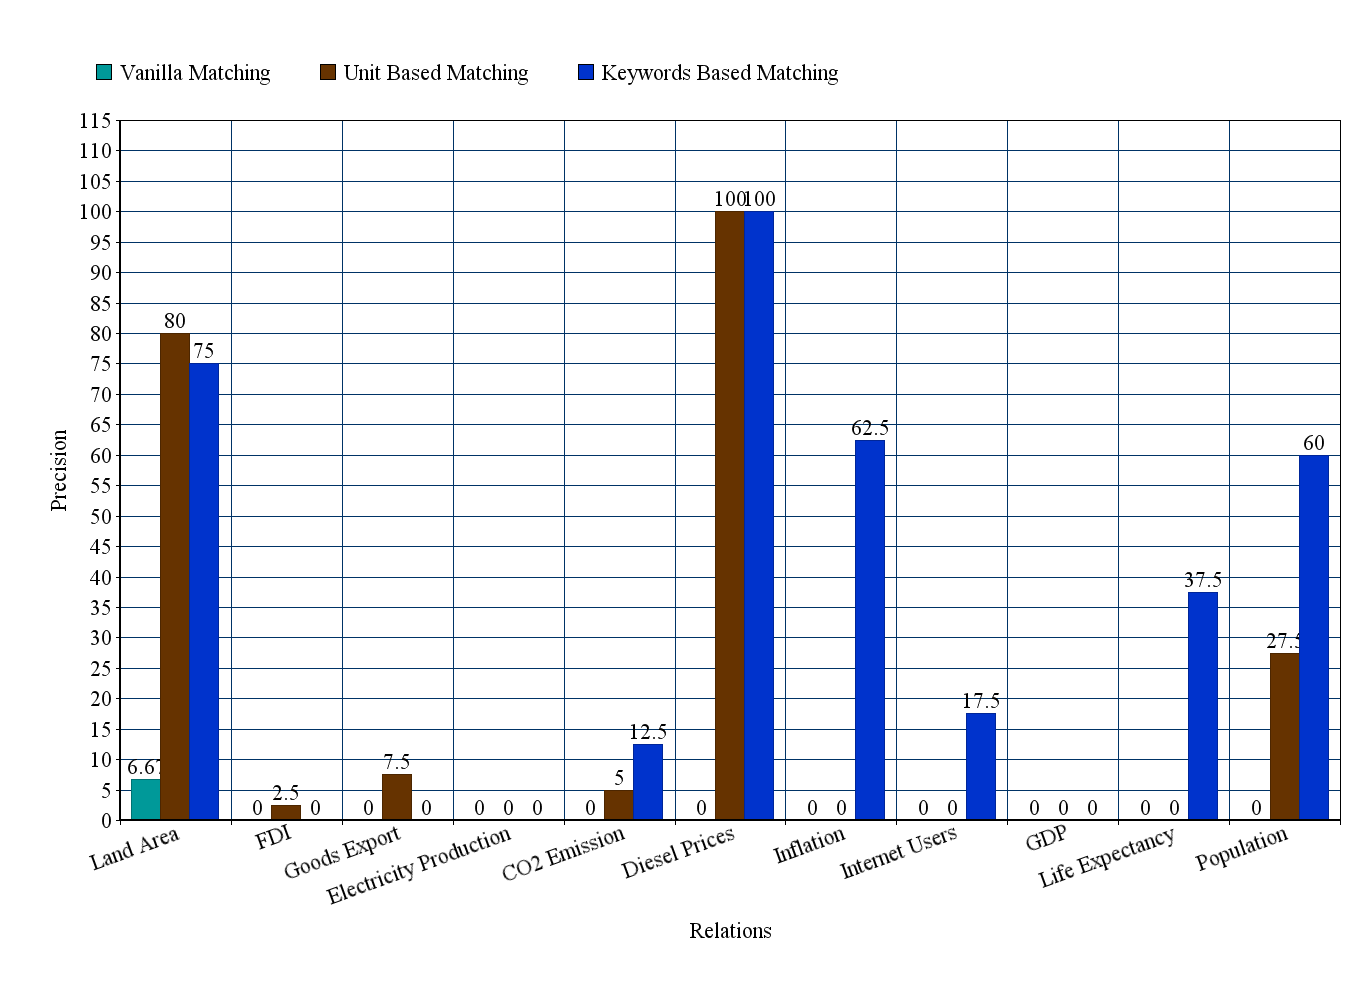
\includegraphics[width = 1.0\textwidth]{images/results}
  \end{figure}
\end{frame}
\begin{frame}{Relative Recall}
\begin{itemize}
 \item Different Heurisitic improved some aspect of matching for distant supervision.  \\~\\
 \item But we need to be careful, that with agressive pruning of incorrect sentences, we are not leaving some good sentences. \\~\\
 \item So for all the Heuristics, we calculate the percentage of true matches that were extracted by each Heuristics. We call this \textbf{Relative Recall}
\end{itemize}
\begin{center}
\begin{tabular}{|l|l|}
 \hline
 Total Sentences for evaluation & 676 \\
 \hline
 Total True Positives & 138 \\
 \hline
 Vanilla Matching & 2 \\
 Units + Distance Based Matching & 79 \\
 Keywords + Units + Distance Based Matching & 112 \\
 \hline
 
\end{tabular}
\end{center}
\end{frame}


%PART 9 : Rule Based Extractions
\section{Dependency Path based Relation Extraction}
\begin{frame}{Dependency Path Based Relation Extraction}{Peculiarity of Numerical Relations}
\begin{itemize}
 \item Analyzing a number of sentences expressing numerical relations lead to several insights as already discussed. \\~\\
 \item \textbf{Units} Are crucial in filtering out candidate relations \\~\\
 \item \textbf{Keywords} We can expect presence of certain keywords that might help in identifying relations. \\~\\
 \item \textbf{Modifiers} A large number of false positives stem out of mentions where a change in the numerical attribute is mentioned.
\end{itemize}

\end{frame}

\begin{frame}{Dependency Path Based Relation Extraction}{Dependencies}
\begin{itemize}
 \item Dependencies: Grammatical relation between two words, governer and dependent. \\
 \item ``The red ball was lost'' \\
\item \begin{itemize}
\item \textbf{amod(ball,3,red,2)} ``Red'' is an adjective for ``ball''
\item \textbf{det(ball,3,The,1)}  ``the'' is a determiner of ``ball''
\item \textbf{nsubjpass(lost,5,ball,3)}	``ball'' is the subject of ''lost''
\item \textbf{auxpass(lost,5,was,4)}	``was''' is an auxiliary of ``lost''
\end {itemize}
\end{itemize}
\begin{figure}[h]
 \centering
 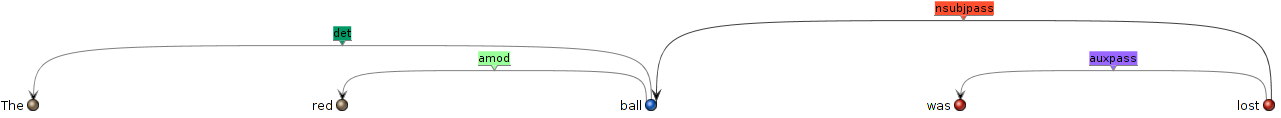
\includegraphics[bb=0 0 1281 118,scale=0.25]{./imgs/dep.png}
 % dep.png: 1281x118 pixel, 72dpi, 45.19x4.16 cm, bb=0 0 1281 118
\end{figure}

\end{frame}

\begin{frame}{Dependency Path Based Relation Extraction}{Technique}
 
\begin{itemize}
 \item Given a Country-Number pair, extract the \textbf{shortest undirected path} between them in the dependency graph.
\end{itemize}
 \begin{figure}[h]
 \centering
 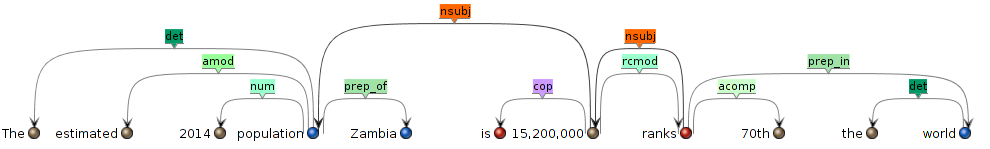
\includegraphics[bb=0 0 990 149,scale=0.3]{./dep.png}
 % dep.png: 990x149 pixel, 72dpi, 34.92x5.26 cm, bb=0 0 990 149
\end{figure}
\begin{itemize}
 \item Path(Zambia - 15,200,000) = \{Zambia, population, 15,200,000\}
  \item For a match, the path:
  \begin{itemize}
   \item \textbf{Should have} one of the keywords
   \item \textbf{Should not have} a modifier
  \end{itemize}
 \end{itemize}
\end{frame}

\begin{frame}{Dependency Path Based Relation Extraction}{Example}
\begin{figure}[h]
 \centering
 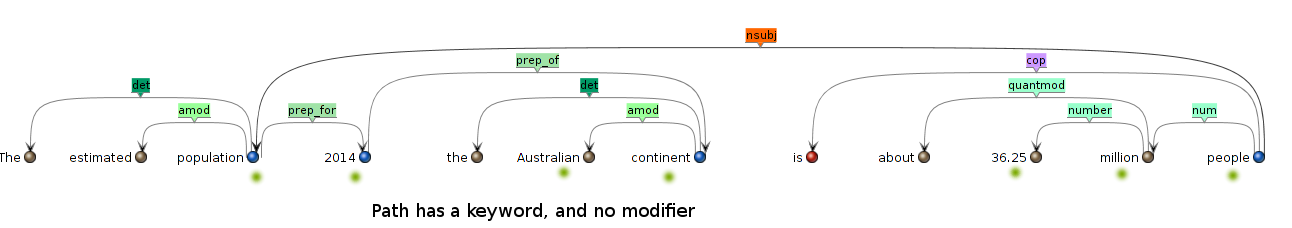
\includegraphics[bb=0 0 1292 228,scale=0.25]{./dep_pos.png}
 % dep_pos.png: 1292x228 pixel, 72dpi, 45.57x8.04 cm, bb=0 0 1292 228
 \caption*{Extracted}
\end{figure}
\begin{figure}[h]
 \centering
 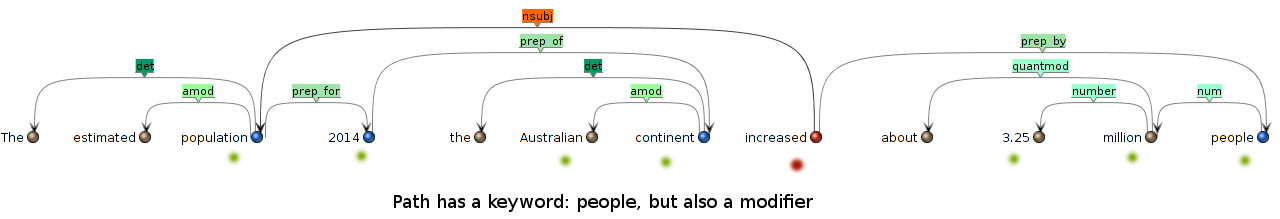
\includegraphics[bb=0 0 1280 219,scale=0.25]{./dep_neg.png}
 % dep_neg.png: 1280x219 pixel, 72dpi, 45.15x7.72 cm, bb=0 0 1280 219
 \caption*{Not Extracted}
\end{figure}

\end{frame}

\begin{frame}{Dependency Path Based Relation Extraction}{Results}
\begin{itemize}
\item The extractor was applied to 30 sentences expressing 23 different relations. \\

\item \resizebox{\linewidth}{!}{% Resize table to fit within \linewidth horizontally
 
\begin{tabular}{|l|l|l|}
\hline
& Relations Present & Relations not Present (False positives) \\
\hline
Extracted & 16 & 17 \\
\hline
Not Extracted & 7 & N/A \\
\hline
\end{tabular}}

 \begin{itemize}
  \item Precision: 48.4\%
  \item Recall: 69.6\%
 \end{itemize}

\item Unit filtering not yet implemented, can be expected to boost precision.
\end{itemize}

\end{frame}

\begin{frame}{Summary}
\begin{itemize}
 \item Out of the box distant supervision for numerical relation extraction is a hopeless cause; Numbers are tricky. \\~\\
 \item Units may help in improving the quality of training data, but will still leave us with plenty of false positives. \\~\\
 \item Numbers are weak entities, can use keywords indicating relations to prune matches. \\~\\
 \item Grammatical structure of sentences expressing numerical relations may be directly exploited, initial results are motivating. \\~\\
\end{itemize}

\end{frame}

\begin{frame}[plain,c]
%\frametitle{A first slide}

\begin{center}
\Huge Thanks!
\end{center}

\end{frame}
\end{document}

